\documentclass[12pt,titlepage, twoside]{article}
\usepackage[utf8]{inputenc}
\usepackage[english]{babel}
\usepackage[titletoc]{appendix}
\usepackage{graphicx}
\usepackage{lscape}
\usepackage{epstopdf}
\usepackage{wrapfig}
\usepackage{comment}
\usepackage{amsmath, amsthm, amssymb}
\usepackage{eqnarray}
\numberwithin{equation}{section}
\numberwithin{figure}{section}
\numberwithin{table}{section}
%\addcontentsline{toc}{chapter}{\listfigurename}
\usepackage{hyperref}
\usepackage{amsfonts}
\usepackage{fixltx2e}
\usepackage{nomencl}
\usepackage{natbib}
\usepackage{setspace}
\usepackage{caption}
\usepackage{subcaption}
%\usepackage[toc,page]{appendix}
\usepackage{fancyhdr}
\usepackage[top = 2cm, bottom = 2cm, outer=2 cm, inner = 3cm]{geometry}
\usepackage{footnote}
\usepackage{mathtools}
\usepackage[export]{adjustbox}

\usepackage{textcomp}

%% for including PDF pages
\usepackage{caption}
\usepackage{lipsum}
\usepackage{boxhandler}
\usepackage{pdfpages}

%% for mathematical fractals and symbosl
\usepackage{physics}

%ťhis three for degrees
\usepackage{amsmath}
\usepackage{breqn}
\usepackage{siunitx}

%% this three for numbering of footnotes
\usepackage{footmisc}
\usepackage{perpage}
\MakePerPage{footnote}

%% for using bibtex
\usepackage{natbib}
%\setcitestyle{numbers,square,sort&compress}


%% for eps
\usepackage{epstopdf}

%\usepackage[numbers,comma,sort&compress]{natbib}
%Calls bibliography commands 
\bibliographystyle{ieeetr}


%\usepackage{blockarray}% http://ctan.org/pkg/blkarray
%\newcommand{\matindex}[1]{\mbox{\scriptsize#1}}% Matrix index


\DeclareMathOperator{\arccosh}{arccosh}
\DeclareMathOperator{\arcsinh}{arcsinh}
\DeclareMathOperator{\arctanh}{arctanh}
\DeclareMathOperator{\arctg}{arctg}
%%\captionsetup[table]{font={stretch=1.2}}     %% change 1.2 as you like
\captionsetup[figure]{font={stretch=1.5}} 

\renewcommand{\listtablename}{Seznam tabulek}
\renewcommand{\listfigurename}{Seznam obrázků}

%\usepackage{stdpage}
\let\abbrev\nomenclature
\renewcommand{\nomname}{List of Abbreviations}
\setlength{\nomlabelwidth}{.25\hsize}
\renewcommand{\nomlabel}[1]{#1 \dotfill}
\setlength{\nomitemsep}{.2cm} \makenomenclature
\newcommand{\Listofabbrev}{
\printnomenclature
\newpage
}
%%%%%%% dvakrat prelozit build.tex a pak spustit makeindex build.nlo -s nomencl.ist -o build.nls a znovu prelozit build.tex %%%%%%%-\parsep

\newcommand{\konv}[1]{\ensuremath{\stackrel{\rm #1}{\longrightarrow}}}
%\topmargin      -3cm \oddsidemargin  -1.5cm \textwidth      19cm
%\textheight     26cm

%************************************************%												%
%			Moje nastavení rozměrů				%
%												%
%************************************************
%\hoffset -1.54cm
%\voffset -0.04pt
%\evensidemargin 3 cm
%\oddsidemargin 2 cm
\topmargin -.5cm
\marginparwidth = 50pt
\marginparsep = 3pt

\textheight 217mm
%\textwidth 165mm

%\renewcommand{\baselinestretch}{1.5}

%************************************
%			REFERENCE				%
%************************************
\bibliographystyle{unsrt}


%************************************************%												%
%		Moje nastavení paragraph				%
%												%
%************************************************
% namísto subsubsubparagraph; není v obsahu, potřeba mezitím enter, jinak to nehodí číslo!

\usepackage{titlesec}

\setcounter{secnumdepth}{4}

\titleformat{\paragraph}
{\normalfont\small\bfseries}{\theparagraph}{1em}{}
\titlespacing*{\paragraph}
{0pt}{1.0ex plus 0ex minus -.5ex}{0.0ex plus 0.0ex}
%{\normalfont\normalsize\bfseries\itshape}
%***********************************
%

%************************************
%		Nedělitelná slova			%
%************************************
\hyphenation{Drucker-Prager}
\hyphenation{Mohr-Coulomb}

\newcommand\cleartooddpage{\clearpage
	\ifodd\value{page}\else\null\clearpage\fi}

\renewcommand{\footnoterule}{%
	\kern -1pt
	\hrule width \textwidth height 1pt
	\kern 2pt
}

%************************************
%			commenting todos				%
%************************************
%\usepackage[colorlinks]{hyperref}
\usepackage[colorinlistoftodos]{todonotes}
\usepackage{verbatim}




%\pagenumbering{roman} % Start roman numbering
\begin{document}




\thispagestyle{empty}
\begin{center}\setstretch{1.0}{
		{\LARGE \textsc CZECH TECHNICAL UNIVERSITY \\[0.3cm]IN PRAGUE}\\[2ex]
		{\LARGE \textsc Faculty of Civil Engineering}\\[2ex]
		{\LARGE \textsc Department of Mechanics}\\
		\vspace{1cm}
		\begin{figure}[ht!]
			\begin{center}
				{
\includegraphics[width=5cm]{lev_novy.eps}}
			\end{center}
		\end{figure}
		\vspace{1cm}
		
		{\textbf {\Huge Bachelor\textquotesingle s Thesis \\[4ex]}
			{\LARGE \bf Computational modeling of thermoset polymers with application to anchors \\[1ex]}
		}
		
		\vfill
		
		{\Large \bf Jan Vozáb }\\ [4ex]
		{\large \bf  Supervisor: Doc. Ing. Jan Vorel Ph.D.}\\[4ex]
		{\Large \bf Prague, 2018  }\\
		\newpage}
\end{center}
\thispagestyle{empty}
\begin{center}\setstretch{1.0}{
		{\LARGE \textsc \mbox{ČESKÉ VYSOKÉ UČENÍ TECHNICKÉ \\[0.3cm] V PRAZE}\\[2ex]
		{\LARGE \textsc Fakulta stavebního inženýrství}\\[2ex]
		{\LARGE \textsc Katedra mechaniky}\\
		\vspace{1cm}
	}
		\begin{figure}[ht!]
			\begin{center}
				{
\includegraphics[width=5cm]{lev_novy.eps}}
			\end{center}
		\end{figure}
		\vspace{1cm}
		
		{\textbf {\Huge Bakalářská práce \\[4ex]}
			{\LARGE \bf Počítačové modelování reaktoplastů používaných v kotevních systémech \\[1ex]}
		}
		
		\vfill
		
		{\Large \bf Jan Vozáb   }\\ [4ex]
		{\large \bf  Vedoucí práce: Doc. Ing. Jan Vorel Ph.D.}\\[4ex]
		{\Large \bf Praha, 2018  }\\
		\newpage}
\end{center}

%\pagenumbering{roman} % Start roman numbering


\setstretch{1.2}{
%\input{zadani}
\includepdf[fitpaper]{zadani.pdf}
\cleardoublepage
\newpage
\null\vfill \thispagestyle{empty}
\noindent {\bf Prohl\' a\v sen\' i:} \\
\\
\\
\\
Prohla\v suji, \v ze jsem svou bakalárskou práci vypracoval samostatn\v e a
pou\v zil jsem pouze podklady (literaturu, projekty, software, atd.) uveden\' e v
p\v rilo\v zen\' em seznamu. \\
\\
\\
\\
Nem\' am z\' ava\v zn\'y d\accent23uvod proti u\v zit\' i tohoto \v skoln\' iho d\' ila ve smyslu \S\,60
Z\' akona \v c. 121/2000 Sb., o pr\' avu autorsk\' em, o pr\' avech souvisej\' ic\' ich s
pr\' avem autorsk\' ym a o zm\v en\v e n\v ekter\' ych z\'akon\accent23u (autorsk\'y z\' akon). \\
\\
\\
\\
\\
{V Praze dne}
\\
\indent\hspace{275pt} Jan Voz\' ab
%
%
%
%
\newpage

\clearpage
%\todo[size=\tiny]{Missing abstracts}
%%%%%%%%%%%%%%%%%%%%%%%%%%%%%%%%%%%%%%%%%%%%%%%%%%%%%%%%%%%%
%% Zacatek vzorove strany %%%%%%%%%%%%%%%%%%%%%%%%%%%%%%%%%%
\thispagestyle{empty}

\noindent {\it Název práce:}\\
{\bf Počítačové modelování reaktoplastů používaných v kotevních sytémech}\\

\noindent
{\it Autor:} Jan Vozáb  \\
\\
\noindent
{\it Obor:}       Konstrukce a dopravní stavby\\
\\
\noindent
{\it Druh práce:} Bakalářská práce\\
\\
\noindent {\it Vedoucí práce:} doc. Ing. Jan Vorel, Ph.D.\\   --------------------------------------------------------------------------------------- \\

\noindent {\it Abstrakt:} 

Reaktoplasty mají v konstrukčním inženýrství důležitou roli. V porovnání s jinými odvětvími, jako je automobilový, letecký a kosmický průmysl, použité reaktoplasty nemusí být vždy v průběhu výstavby plně vytvrzené. Z tohoto důvodu může docházet ke změnám vlastností materiálu v důsledku dodatečného vytvrzování. 

Hlavním cílem této práce je vytvoření numerického modelu, který zachycuje dostatečně přesně vývoj materiálových vlastností a chování reaktoplastů při mechanickém zatěžování. 

Model v této práci je složen ze dvou částí. První je model vytvrzování, který zohledňuje vývoj materiálových parametrů v závislosti na teplotě a času. Jako druhý je použitý elasto-plastický model Drucker-Prager, kterýje využit na popis chování materiálu při mechanickém zatěžování.
\\
\\

\noindent {\it Klíčová slova:} dodatečné vytvrzování, reaktoplasty, Drucker-Prager, metoda konečných prvků

 \newpage
\thispagestyle{empty}
 \noindent
{\it Title:}\\
{\bf Computational modeling of thermoset polymers with application to anchors}\\

\noindent
{\it Autor:} Jan Vozáb \\
 
--------------------------------------------------------------------------------------- \\

\noindent {\it Abstract:} 
Compared to their classical appearance in the aerospace or automotive industry, in civil engineering applications they typically do not reach a fully cured state during construction. Therefore, the material may undergo post-curing causing a significant change in material parameters. The main aim of this work is to create a numerical model that describes sufficiently precisely the evolution of material properties and the behavior of thermosetting polymers during mechanical loading. The model in this thesis is composed of two parts. The first is a curing model that takes into account the development of material parameters in relation to temperature and time. The second is the elasto-plastic model Drucker-Prager, which is used to describe the behavior of the material during mechanical loading.
\\
\\

\noindent 
{\it Key words:} material curing, thermosetting polymers, Drucker-Prager, finite element method
%% Konec vzorove strany %%%%%%%%%%%%%%%%%%%%%%%%%%%%%%%%%%%%
%%%%%%%%%%%%%%%%%%%%%%%%%%%%%%%%%%%%%%%%%%%%%%%%%%%%%%%%%%%%

%\end{document}

\newpage\null \vfill \noindent\thispagestyle{empty}{\bf\Large
Acknowledgment}
\bigskip


I would like to say thank to my supervisor, Doc. Ing. Jan Vorel, Ph.D., for his time, patience and for incessantly explaining the same things to me all over again. I would like to thank to my friends and classmates for their support and continuous motivation. Great thanks also belong to my family and especially my girlfriend Radka Sochorová for their psychical support for the duration of making this thesis. 

\newpage


}

\setstretch{1.35}{

\clearpage
\tableofcontents
\pagestyle{plain}
\listoffigures
%\listoftables
}
\newpage 

\newgeometry{top=2cm,bottom=2cm,outer=2cm,inner=3cm,includeheadfoot}

\pagestyle{fancy}
\fancyhead[RO,LE]{}
\fancyhead[RE]{\leftmark}
\fancyhead[LO]{\rightmark}
\renewcommand{\headrulewidth}{0pt}

\setstretch{1.20}{

%\pagenumbering{arabic} % Switch to normal numbers
%\setcounter{page}{1}

%\cleartooddpage
\cleardoublepage
\section*{Introduction}
\addcontentsline{toc}{section}{\protect\numberline{}Introduction}
\indent

In the last century construction engineering as well aerospace engineering  were dominated by the materials steel, aluminum, and concrete. But especially in last decade civil engineers more than ever faced often contradictory demands for designing larger, safer and more durable structures at shorter time and lower costs. This lead to improvement of old and designing of new materials. Composites are a key element of those new designs.

Composite materials often combine positive characteristic properties from more, typically two, different materials which result to better material properties. In many cases these combine a load carrying constituent, typically in the form of carbon or glass fibers, bonded to the cement or polymer based matrices. Their applications can be found in transportation as well as in civil engineering fields. In the aerospace industry we can found entire structural members made of composite materials, but in the building industry we can find the use of polymer-based composites is limited. A typical area are members applied to existing concrete or masonry such as adhesive anchors. The commonly used polymers are typically utilized, exothermically reacting, thermosets, e.g. epoxies or vinyl-esters. They have high filler content (including even cement and water). They have uncertain curing level and the mechanical properties due to the environmental conditions (a fully cured state is not usually reached).

Also a large range of working temperatures, which are typically expected during the lifetime leads to post-curing and related changes in mechanical properties. These changes highly impact in particular structures under sustained or cyclic loads. For these challenges, the characterization of this type of materials is in high demand.  
%\clearpage
%
\mbox{}
\thispagestyle{empty}
\clearpage

\section{Introduction}

In the last century construction engineering as well aerospace engineering  were dominated by the materials steel, aluminum, and concrete. But especially in last decade civil engineers more than ever faced often contradictory demands for designing larger, safer and more durable structures at shorter time and lower costs. This lead to improvement of old as designing new materials. Composites are a key element of those new designs. \todo[size=\tiny]{pokus}

Composite materials often combine positive characteristic properties from more, typically two different materials which result to better material properties. In many cases these combine a load carrying constituent typically in the form of carbon or glass fibers bonded to the cement or polymer based matrices. Their applications can be found in transportation as well in civil engineering fields. In the aerospace industry we can found entire structural members made from composite materials, but in the building industry is using of polymer-based composites limited. A typical area are members applied to existing concrete or masonry such as adhesive anchors. The commonly used polymers face challenges as:

\begin{itemize}
	\item typically utilized exothermically reacting thermosetting polymers, e.g. epoxies or vinyl-esters, with defined post-curing,
	\item high filler content, including even cement and water,
	\item uncertain curing level and the mechanical properties depending on the environmental conditions (a fully cured state is not usually reached).
\end{itemize} 

Also a large range of working temperatures, which are typically expected during the lifetime leads to post-curing and related changes in mechanical properties. These changes highly impact in particular structures under sustained or cyclic loads. For these challenges, the characterization of this type of materials is in high demand.  

\cleardoublepage
%\input{./kapitoly/kapitola20}

\cleardoublepage
%\mbox{}
%\thispagestyle{empty}

\thispagestyle{plain}
\section{Anchor systems}
An anchor is a steel element either cast into concrete or post-installed into a hardened concrete member and used to transmit applied loads, including headed bolts, hooked bolts (J- or L-bolt), headed studs, expansion anchors, or undercut anchors \cite{anchors-ACI-318M}. Anchors are typically used to connect structural elements or to fix non-structural components (or systems) to the structures. 

\begin{figure}[h!]
	\centering
	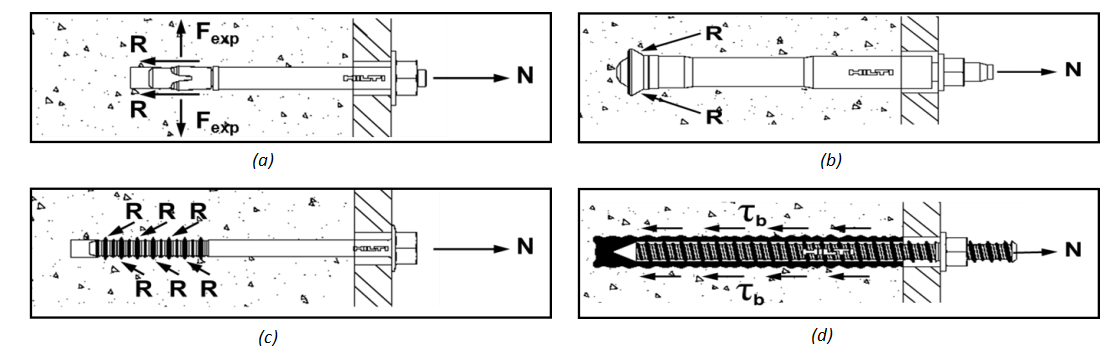
\includegraphics[width=0.9\textwidth]{obrazky/post_installed_anchor_types_repaired.png}
	\caption[Types of post-installed anchors with different load transfer mechanism]{Types of post-installed anchors with different load transfer mechanism ($R$ is direction of reaction force, $N$ is loading of anchor and $F_{exp}$ represent expansion force) \cite{hilti_anchors}: a) friction (micro-keying); b) keying (bearing/undercut); c) keying (screw-type); d) adhesion (bonding).}\label{obr:Post_installed_anchors}
\end{figure}

\subsection{Load transfer mechanisms}
In the Fig. \ref{obr:Post_installed_anchors} we can see different types of load transfer mechanisms. The choice of a  used mechanism affects future method of installation, resilience to different types of loading and even curing time, which some anchors need before loading. Each anchor type is described below in detail \cite{hilti_anchors}. 


\begin{itemize}
	\item \textit{Friction mechanism:}	
	As the name implies, the primary transfer mechanism is friction and it results in bonding from expansion forces between the anchor and the primary structure (Fig. \ref{obr:Post_installed_anchors}a). Frictional force is proportional to the magnitude of expansion stresses generated by the anchor.The expansion is caused by a controlled torque during casting and even, in some cases, later adjusted for changes in the state of the base material.
	
	\item \textit{Keying mechanism:}	
	This transfer principle rely on the interlock of the anchor with deformations in the hole wall to resist external loading (Fig. \ref{obr:Post_installed_anchors}b,c). The bearing stresses created in the base material in the interface with the anchor bearing surface can rise to high values. This type of anchors offers good resilience to variations in the base material conditions and thus represent one of the most robust solutions for anchor designs. 
	
	\item \textit{Bonding mechanism:}	
	This mechanism relies on adhesion between the concrete and the anchor created by adhesive (Fig. \ref{obr:Post_installed_anchors}d). The degree of bonding available is depending on the conditions of the whole wall at the time of anchor installation and used type of adhesive material. This type of mechanism offers flexibility and high bond resistance for a wide variety of anchoring applications. 
\end{itemize}

\begin{figure}[h!] 
	\centering 
	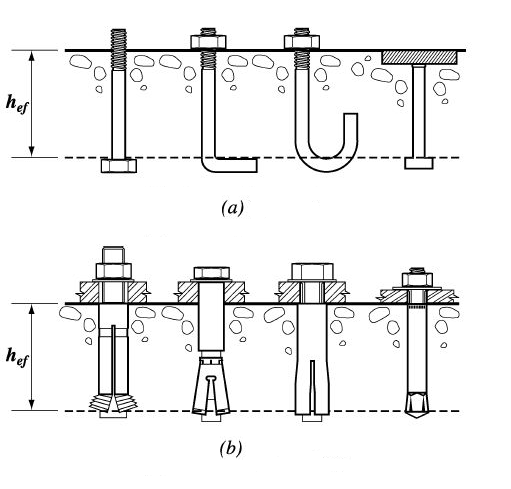
\includegraphics[width=0.6\textwidth]{obrazky/anchor_types_repaired.png} 
	\caption[Types of anchors]{Types of anchors ($h_{ef}$ is effective anchor length) \cite{anchors-ACI-318M}: a) cast-in-place; b) post-installed.}\label{obr:Anchors} 
\end{figure} 


\newpage
\subsection{Types of anchors}
\indent

Anchors can be divided by the load transfer mechanism, but another important criterion before choosing a specific solution is the installation time, when an anchor is fixed. As you can see in Fig. \ref{obr:Anchors}, anchors can be divided into two main groups: $\mathrm{a)}$ cast-in-place and $\mathrm{b)}$ post-installed. 


\subsubsection{Cast-in-place anchors}
The cast-in-place anchors are the simplest type of anchor. As the name suggests, these anchors are cast in the wet concrete or with reinforcement of concrete. In the Fig. \ref{obr:Anchors} we can see that designs can consist of a standard bolt with a hexagonal head (hex head bolt $\mathrm{(a.1)}$), “hooked” J bolts  $\mathrm{(a.2)}$ and L bolts $\mathrm{(a.3)}$. These anchors are very strong, and can be used in most anchor applications, butx they are also difficult to cast. Therefore, they are recommended when the large embedment length or the high tensile strength are required.

\subsubsection{Post-installed anchors}
Post-installed anchors are in general, technically sophisticated products, but are easy to install and provide more variability than cast-in anchors like headed studs. They can be cast into already hardened concrete as well as into masonry but they are a lot more sensitive to the boundary conditions than cast-in-place anchors. Most of the commercially available post-installed anchor products can be assigned to one of the major types which are categorized according to their load transfer mechanism (Fig. \ref{obr:Post_installed_anchors}).


\subsubsection{Types of post-installed anchors}
Four main groups of post-installed anchors based on a load transfer mechanism and method of installation can be found in the literature \cite{hilti_anchors}.
 
	\begin{itemize}

	\item \textit{Expansion anchors}, which have the primary principle of load transfer mechanism based on the friction, bearing or both. Anchors are inserted into a drilled hole in the hardened concrete or masonry. Main advantages are immediate load transfer and no temperature restrictions, but on the other hand they are not the best in transfer capacity. 

	\item \textit{Undercut anchors} create holding strength with the mechanical interlock provided by undercutting the concrete near the back of the hole. This is achieved by a special tool or by the anchor itself during installation. The main load transfer mechanism is keying. This type of anchors have benefits like high transfer capacity, immediate loading transfer, or no temperature restrictions, but they are more difficult to install. 

	\item \textit{Screw anchors} are inserted into drilled hole with a diameter typically smaller than the anchor. Typical load transfer mechanism is keying. The advantages are immediate full loading transfer or no temperature restrictions, but the anchors can reach just low loading capacity.

	\item \textit{Adhesive anchors} are post-installed into drilled hole in hardened concrete, masonry or stone. Loads are transferred to the base material by the bond created by an adhesive on the anchor, so the load transfer mechanism is a bonding. Advantages of this type of anchor are a simple installation and a high capacity. Main disadvantages are temperature restrictions and a curing time needed before loading. But full curing state is not typically reached. Modeling partly cured adhesive is difficult due to a large number of variables such a loading history, time, temperature, even humidity. Modeling of this adhesive material is the main target of this thesis.
\end{itemize} 

\subsection{Loading and failure modes}
An anchor is in most cases loaded in tension and shear. This loading checks all parts of anchor, even the base material. According to a norm \cite{anchors-ACI-318M}, the strength design of anchors shall be based either on computation using design modes that satisfy requirements of the norm, or on test evaluation using the 5 percent fractile of test results for the following:

\begin{itemize}
	\item steel strength of anchor in tension,
	\item steel strength of anchor in shear, 
	\item concrete breakout strength of anchor in tension,
	\item concrete breakout strength of anchor in shear,
	\item pullout strength of anchor in tension (including adhesive), 
	\item concrete side-face blowout strength of anchor in tension,
	\item concrete pry out strength of anchor in shear.
\end{itemize} 

\begin{figure}
	\centering
	\begin{subfigure}{.5\textwidth}
		\centering
		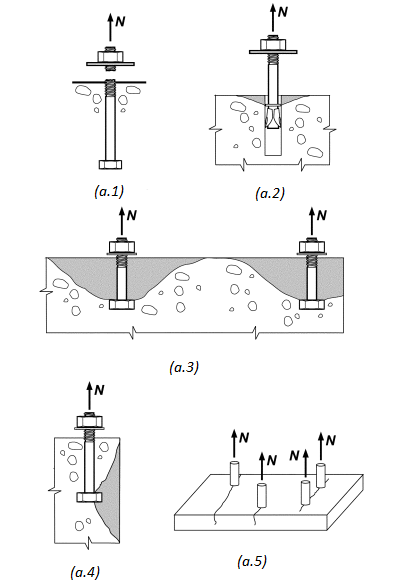
\includegraphics[width=.9\linewidth]{obrazky/failure_models_tensile.png}
		\caption{tensile loading, where $N$ is tensile force}
		\label{obr:tensile_loaded}
	\end{subfigure}%
	\begin{subfigure}{.5\textwidth}
		\centering
		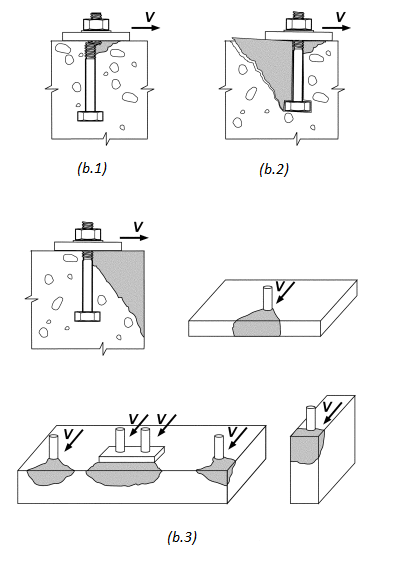
\includegraphics[width=.9\linewidth]{obrazky/failure_models_shear.png}
		\caption{shear loading, where $V$ is shear force}
		\label{obr:shear_loaded}
	\end{subfigure}
	\caption[Failure modes of anchors]{Failure modes of anchors \cite{anchors-ACI-318M}: a.1) steel failure; a.2) pullout; a.3) concrete breakout; a.4) side-face blowout; a.5) concrete splitting; b.1) steel failure preceded by concrete spalling; b.2) concrete pryout for anchors far from a free edge; b.3) concrete breakout.}
	\label{obr:failture_models}
\end{figure}


\begin{figure}[h!]
	\centering
	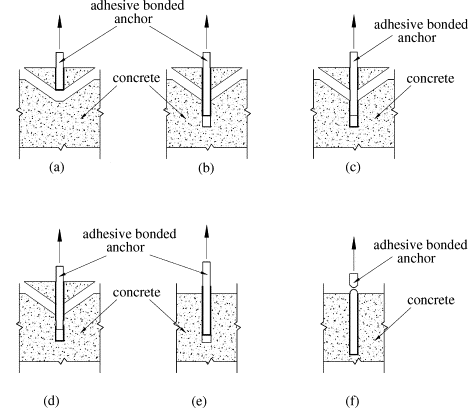
\includegraphics[width=0.6\textwidth]{obrazky/adhesive_failture_models_repaired.png}
	\caption[Failure modes of adhesive anchors in tensile]{Failure modes of adhesive anchors in tension \cite{adhesive_anchors}: a) concrete cone failure; b) adhesive/concrete interface bond failure; c) steel/adhesive interface bond failure; d) mixed bond failure; e) bond failure; f) steel failure.}
	\label{obr:failture_adhesive_models}
\end{figure}
 
These failure modes are shown in Fig. \ref{obr:failture_models}. However, adhesive anchors have even more complicated failure modes due to a full length bond, which can be damaged in different ways, see Fig. \ref{obr:failture_adhesive_models}.


\cleardoublepage
%\mbox{}
%\thispagestyle{empty}
%\newpage
\thispagestyle{plain}
\section{Thermoset polymers}\label{sec:thermo_polymers}

Plastic materials may be classified into two main categories based on their response to temperature: thermoplastic and thermosetting polymers. A thermoplastic materials behaves like fluid above a certain temperature level, but the heating of a thermosetting material leads to its degradation without its going through a fluid state. This classification is not restricted to plastic materials but may also be extended to the behavior of coating, adhesives and several other categories. This is why we find it better to use the term \textit{thermoset polymers}, which implies the different ways in which these materials are used and adds the fact that a constitutional repeating unit (CRU)\footnote{The smallest constitutional unit which repetition constitutes a regular macromolecule, a regular oligomer molecule, a regular block or a regular chain.} is present in their chemical structure. These materials are also referred to as \textit{thermoset resins}, which is a vaguer definition that may be applied to the starting monomers or oligometric precursors, as well as to the final materials \cite{thermosetting_polymers}. 

\subsection{Thermoset polymers used with anchors}\label{subsec:polymers_in_anchors}
Utilized mortars, with reference to the anchor systems, are composed of thermoset polymers (e.g. vinyl-ester based and epoxy systems) and high filler content (e.g., sand, stone, cement) of about 40\%.

\subsubsection{Vinyl-ester systems}\label{subsec:vinyl_ester}
Vinyl-ester based systems are more pricey than epoxy systems, but not that much. It is a hybrid form of polyester resin which has been toughened with epoxy molecules within the main molecular structure and offers better resistance to moisture absorption, but it's downside is sensitivity to mixing, handling, atmospheric moisture and temperature sensitivity (sometimes it just will not cure). The toughening effect of the resin modifications makes a better resistance to micro fracturing and some of the secondary functionality of the backbone assisting in adhesion to substrates. Vinyl-esters are capable of forming secondary bonds around $3400~\mathrm{kPa}$. Vinyl-esters definitely represent an improvement over polyesters when considering standard peroxide curing, however adhesion to dissimilar and already cured substrates is still far below perfect and many vinyl-ester hulls suffer similar massive delamination of the hull skins from core and bulkhead substrates. It is also known that vinyl-ester resins bond very well to fiberglass, but offer a poor bond to kevlar and carbon fibers.  Open surface curing vinyl-esters require a surfacing agent and subsequent applications require careful surface preparation if reasonable adhesion is to be achieved \cite{thermosetting_polymers}.

\subsubsection{Epoxy systems}\label{subsec:epoxy_systems}
Epoxy systems in all categories of work will realize the greatest degree of bond strength, water-resistance and toughness. Well-reinforced epoxy repair will tenaciously hold to the substrate with almost $14 000~\mathrm{kPa}$ strength. In areas that must be able to flex and strain with the fibers without micro-fracturing, epoxy resins offer much greater capability. Cured epoxy tends to be very resistant to moisture absorption. Epoxy resin will bond dissimilar or already-cured materials which makes repair work that is  very reliable and strong. It actually bonds to all sorts of fibers very well and also offers excellent results in repair-ability when it is used to bond two different materials together. New generation of epoxy systems feature many of the advantages of low viscosity and accurately tailored gel and cure times \cite{thermosetting_polymers}. 

\subsection{Numerical description of thermoset polymers}\label{sec:poly_complexity}
In order to describe thermoset polymers, there are more degrees of complexity (in this thesis two), depending on the number of variables taken into account in constitutive equations under consideration (see also \cite{thermosetting_polymers}). 
\begin{itemize}
	
	%%%%%%%%%%%%%%%%%%%%% FIRST LEVEL %%%%%%%%%%%%%%%%%%%%%%
	\item 
	\textit{First level}, where these equations could take into account only two variables: the stress $\sigma$ and the strain $\varepsilon$:
	
	\begin{equation}\label{eq2:first_level}
		f(\sigma,\varepsilon)=0.
	\end{equation}
	
	This limits model mechanical simulation for relatively sharp intervals of time and temperature. It can be considered sufficient for a description of material behavior at low strains. For the isotropic material, moduli are defined by the following equations:
	
	\begin{equation}\label{eq:basic_moduli}
		E = 3K(1-2\nu); ~~G=\dfrac{3}{2}\dfrac{(1-2\nu)}{(1+\nu)};~~ K=\frac{E}{2(1+\nu)},
	\end{equation}
	
	where $E$ is the elastic (Young) modulus, $G$ means the shear (Coulomb) modulus, $K$ represent the bulk modulus, and $\nu$ is Poisson's ratio. $E$ can be obtained from a uniaxial tensile test $(E=\sigma/\varepsilon)$, or a uniaxial compressive test, or flexural test; $G$ can be determined from a shear test $G=s/\gamma$, where $s$ is the shear stress and $\gamma$ is the shear strain; K can be determined from a compressibility test, 
	
	\begin{equation}\label{eq:K_moduli}
		K=\left(\dfrac{1}{V}\dfrac{dV}{dp}\right)^{-1},
	\end{equation}
	
	where $V$ is the volume and $p$ is the hydrostatic pressure; and $\nu$ can be figured out from two independently determined values of modulus, or from a tensile test using a bidimensional extensometer. 
	
	\begin{figure}
		\centering
		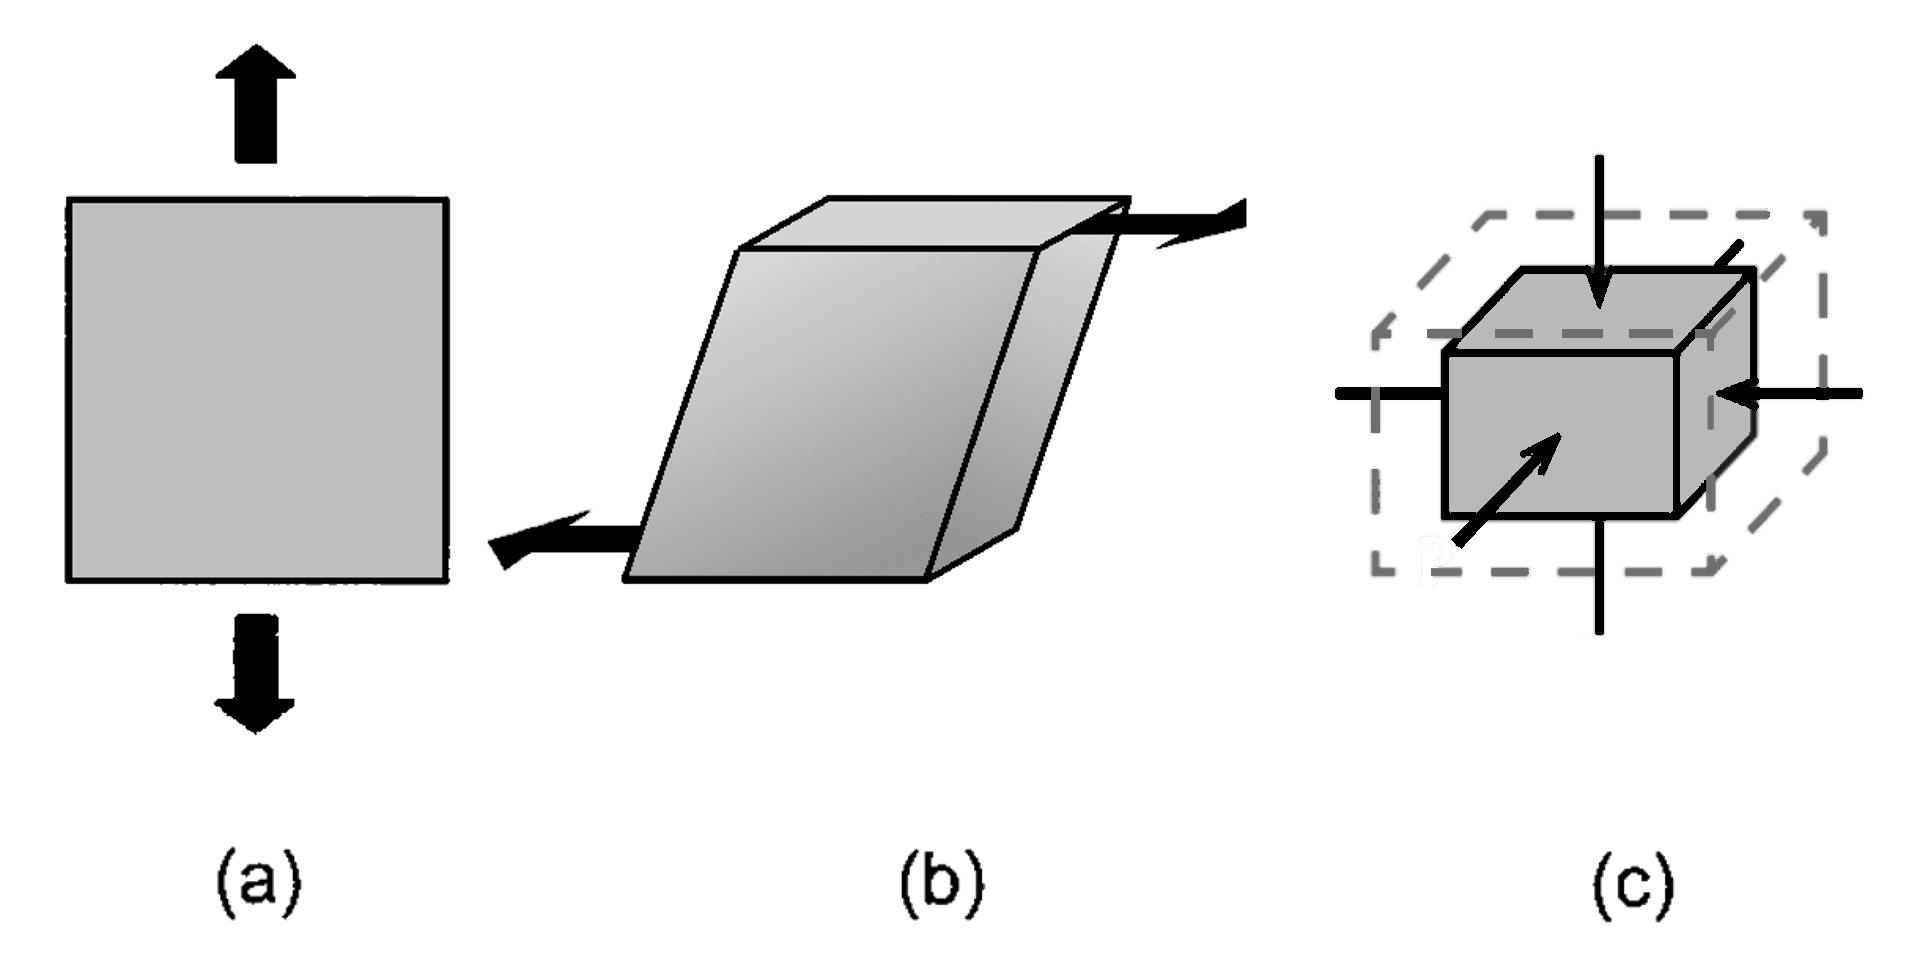
\includegraphics[width=0.7\linewidth]{obrazky/mechanical_tests}
		\caption[Mechanical tests to determine E, K, G moduli]{Mechanical tests to determine (a) E; (b) G; (c) K.}
		\label{fig:mechanicaltests}
	\end{figure}

	%%%%%%%%%%%%%%%%%%%%% SECOND LEVEL %%%%%%%%%%%%%%%%%%%%%%
	\item
	\textit{Second level}, where the constitutive equations must involve two (or more) additional variables. For instance:
	
	\begin{equation}\label{eq:second_level}
		f(\sigma,\varepsilon,\dot{\varepsilon},T, t, c, \Theta)=0,
	\end{equation}
	
	where $\dot{\varepsilon}$ is the strain rate, $T$ means the temperature, $t$ represents time , $c$ is the moisture content and $\Theta$ stands for the mechanical dilatation.	These new variables are necessary for, e.g., addition of viscoelastic behavior into the material model. This behavior is linked to the molecular motions, which are important in the glassy domain (in the Fig. \ref{fig:effectoncrosslinkdensity} between boundaries $\alpha$ and $\beta$). Also they affect the behavior in the glass transition region (around boundary $\alpha$). High influence on the behavior also have thermo-mechanical history due to an anchor installation and a physical aging of the material. The relationships that describe the effects of $\dot{\varepsilon}$, $\dot{\sigma}$, $T$, $t$, $c$ and $\Theta$ on the previously defined elastic properties are also needed if the extensive model is adopted.
	
	\begin{figure}
		\centering
		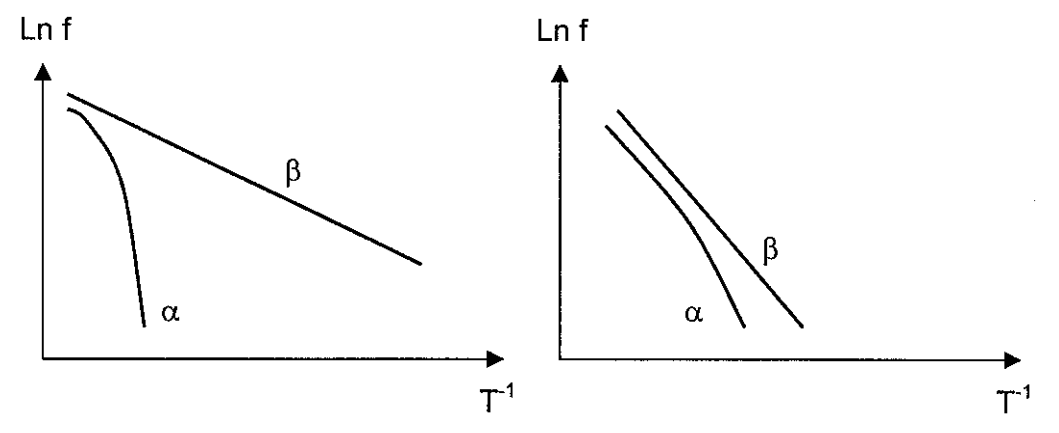
\includegraphics[width=0.8\linewidth]{obrazky/effect_on_cross_link_density}
		\caption[Shape of relaxation maps]{Shape of relaxation maps: dependence of $\ln f$ (frequency) to reciprocal temperature for coordinates of transitions $\alpha$, $\beta$: (a) - polymers having their $\alpha$ and $\beta$ transitions well separated; (b) - polymers with close $\alpha$ and $\beta$ transitions}
		\label{fig:effectoncrosslinkdensity}
	\end{figure}
	
	In the literature we can find three major experimental methods for mechanical characterization in this region, which correspond to particular solutions of the material's state equation: 
	
	\begin{itemize}
		\item Static tests: $\varepsilon = \varepsilon_{0} = constant$ for relaxation, or $\sigma = \sigma_{0} = constant$ for creep. 
		
		\item Monotonous tests with loading rate $\dot{\varepsilon}$, or $\dot{\sigma} = constant$ (for example tensile tests): 
		
		$\dot{\varepsilon} = \dfrac{1}{l}\dfrac{dl}{dt}$
		
		\item dynamic tests: $\varepsilon = \varepsilon_{0} \sin(\omega t)$, or $\sigma = \sigma_{0} \sin(\omega t)$
	\end{itemize}
	
	Polymers are generally assumed to obey the Boltzmann superposition principle in the region of small strains. When there are changes of loading conditions, the effects of these changes are additive when the corresponding responses are considered at equivalent times. For example, if different stresses $\sigma_{0}$, $\sigma_{1}$, $\sigma_{2}$,...$\sigma_{i}$ are applied at different times $0$, $t_{1}$, $t_{2}$,...$t_{i}$, respectively, the final strain is
	
	\begin{equation}\label{eq2:boltzmann_eps}
		\varepsilon(t) = J(t)\sigma_{0} + J(t-t_{1})\sigma_{1}+J(t-t_{2})\sigma_{2}+\cdots+J(t-t_{i})\sigma_{i}
	\end{equation}
	
	where $J(t)$ is the time-dependent creep compliance.
	
	In the same manner, if different strains $\varepsilon_{0}$, $\varepsilon_{1}$, $\varepsilon_{2}$,...$\varepsilon_{i}$ are applied at times $0$, $t_{1}$, $t_{2}$,...$t_{i}$, the final stress is 
	
	\begin{equation}\label{eq2:boltzmann_sig}
	\sigma(t) = E(t)\varepsilon_{0} + E(t-t_{1})\varepsilon_{1}+ E(t-t_{2})\varepsilon_{2}+\cdots+E(t-t_{i})\varepsilon_{i}
	\end{equation}
	
	where $E(t)$ is the time-dependent relaxation modulus. It is generally effective to use dynamic tests to obtain $J(\omega)$ or $E(\omega)$, and then with using mathematical transformations determine $J(t)$ or $E(t)$.
	
	Ordinary, polymers obey a time-temperature superposition principle:
	
	\begin{equation}\label{eq2:shift_factor}
		P_{r}(t,T) = P_{r} \left(\dfrac{t}{a_{T}}, T_{r}\right)
	\end{equation}
	
	where $P_{r}$ is function of $T_{r}$ and $a_{T}$. In Eq. (\ref{eq2:shift_factor}), $T_{r}$ is a reference temperature and $a_{T}$ is a thermal shift factor that depend on temperature, humidity and mechanical dilatation. Polymers are interesting in that $a_{T} = f(T, c, \Theta)$ takes different mathematical forms below and above glass transition temperature $T_{g}$.
	
\end{itemize}


\subsection{Material properties}\label{subsec:mat_proper}
\indent

Material properties, needed for studying model performance of thermoset polymers, are directly connected to degree of complexity which is being investigated. As you can see in Sec. \ref{sec:poly_complexity}, in the first level basic mechanical properties are needed, e.g. Young's modulus $E$ and Poisson's ratio $\nu$. But such low number of material properties makes model limited to relatively sharp intervals of time and temperature, and functioning at low strains.

A higher level of complexity is needed to capture the complicated material behavior. This leads to the more specific material properties, which include yielding and fracture properties, volumetric properties, cohesive properties, glass transition properties, crosslink density, chain mobility, viscoelastic properties,curing degree and aging of the material. Some of them are described below in a more detail.	

\begin{itemize}
	\item 	Yielding properties define boundary between reversible and permanent deformation, but also behavior of the material over this boundary. In normal conditions, the material must be used below the yield boundary, often called the elastic limit of material. If the stress goes beyond its yield boundary, the ultimate fracture stress (lost of material integrity) becomes important. Then we need specific theoretical and experimental tools, e.g., fracture mechanics, to study these phenomena.
	
	\item Volumetric properties include free volume, density, packing density and expansion. Free volume is an intrinsic property of the polymer matrix and is created by the gaps left between entangled polymer chains. It can affect absorption and diffusion of the molecules in polymers.
	
	\item Cohesive properties are represented by the cohesive energy as the whole energy of intermolecular interactions, which is easy to determine from calorimetric measurements\footnote{For small molecules}, and cohesive energy density.
	
	\item Glass transition is a catastrophic softening of the material, when temperature is higher then the glass transition temperature $T_g$. Also has influence to the curing process due to its exothermal behavior. 
	
	\item Viscoelastic properties include creep and relaxation properties, which describe connections between the stresses and strains with respect to time. Creep means increasing of the strains in time with constant stress and relaxation means reduction of the stresses under constant strains. 
	
	\item Curing degree defines change of the material from the liquid to the glassy state. Note that bonded anchors have an uncertain curing degree of the mortar when they are loaded.
	
\end{itemize}



\cleardoublepage
%\mbox{}
%\thispagestyle{empty}
%\newpage
\section{Computational modeling}
\indent

For modeling of thermosetting polymers we have used three methods of numerical solution. Firstly, the Drucker-Prager plasticity model used to simulate the mechanical behavior. The reason for selection that basic numerical model was an impulse to learn implementing in C++ programming language into FEM software, so it can by used to the numerical simulations of the anchors, which could be compared to real test results. Implementing into used FEM solver Mars \cite{mars} was way more complicated due to object oriented programming language. Second method was a curing model, which already was completed into Mars solver and were used to describe time dependent behavior of material. At last we used model created by serially connected curing model to Drucker-Prager model, again in Mar solver, which lead to more real behavior of material due to including dependence on time into plasticity mechanical behavior. All methods are described below in detail.

\subsection{Finite element method}
\indent

Finite element method is a numerical solution used for the simulation of stresses, strains, natural frequency, heat transition, electromagnetic effects, flow of fluids, etc., on a created physical model. The main principle is in discretization of continuum to finite number of elements, where are investigated parameters examined on each element. FEM is used typically for inspection an already modeled structures or for determination of critical region of the structure. Through principles of this method were developed in first half of twentieths century, its massive expansion occurred with succession of a modern computer technologies. 
\newpage
\subsection{Vectors and matrices}
\indent

Before proceeding with te actual formulation of individual constitutive models, we first define the following matrices and vectors frequently used in this chapter:

\begin{equation}
	\boldsymbol{m} = \lbrace 1/3,1/3,1/3\rbrace ^T,
\end{equation}


\begin{equation}
	\boldsymbol{P} = \mqty[	2/3 & -1/3 & -1/3 & 0 & 0 & 0\\ 
				-1/3 & 2/3 & -1/3 & 0 & 0 & 0\\
				-1/3 & -1/3 & 2/3 & 0 & 0 & 0\\
				0 & 0 & 0 & 2 & 0 & 0\\
				0 & 0 & 0 & 0 & 2 & 0\\
				0 & 0 & 0 & 0 & 0 & 2\\],	\boldsymbol{Q} = \mqty[	1 & 0 & 0 & 0 & 0 & 0\\
				0 & 1 & 0 & 0 & 0 & 0\\
				0 & 0 & 1 & 0 & 0 & 0\\
				0 & 0 & 0 & 1/2 & 0 & 0\\
				0 & 0 & 0 & 0 & 1/2 & 0\\
				0 & 0 & 0 & 0 & 0 & 1/2\\],
\end{equation}





\subsection{Drucker-prager model of plasticity}\label{sec:drucker-prager_introduction}
\indent

If we have results of laboratory tests ploted in effective rather than total stress, then the failure criterion becomes dependent on the hydrostatic or mean stress. Then is appropriate to use Drucker-Prager yield criterion, which describes such dependence. Drucker-Prager model of plasticity extend von Mises model by including mean stress (first invariant of the stress tensor) into the yield surface equation. Unlike Mohr-Coulomb model is Drucker-Prager yield criterion smooth and in space of the principal stresses have form of cylindrical cone, because of that is sometimes is Mohl-Coulomb model replaced with Drucker-Prager and as you can see in the Fig. \ref{obr:F1}, parameters are adjusted to fit or inscribe to Mohr-Coulomb model. The main advantage of that replace is about difficult return to the yield of plasticity with Mohr-Coulomb model due to its corners, which are not included in Drucker-Prager model. Definition and calculation of Drucker-Prager model in this thesis is based on \cite{geofem}.   

\begin{figure}[h!]
	\centering	
	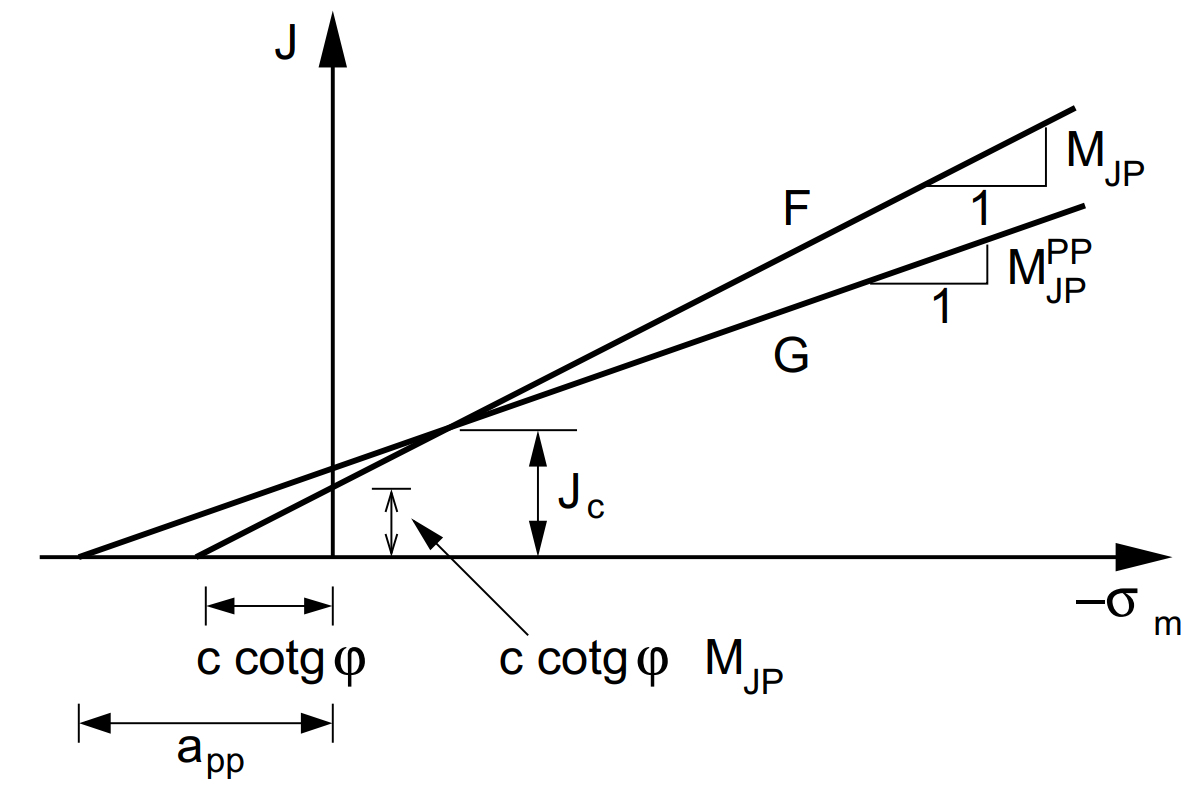
\includegraphics[width=0.7\textwidth, angle=0]{obrazky/drucker_prager_meridian.png}
	\caption[Drucker-Prager yield criterion on meridian plane $T$]{Drucker-Prager yield criterion in meridian plane \cite{geofem}.} \label{obr:M1}
\end{figure}

\begin{figure}[h!]
	\centering	
	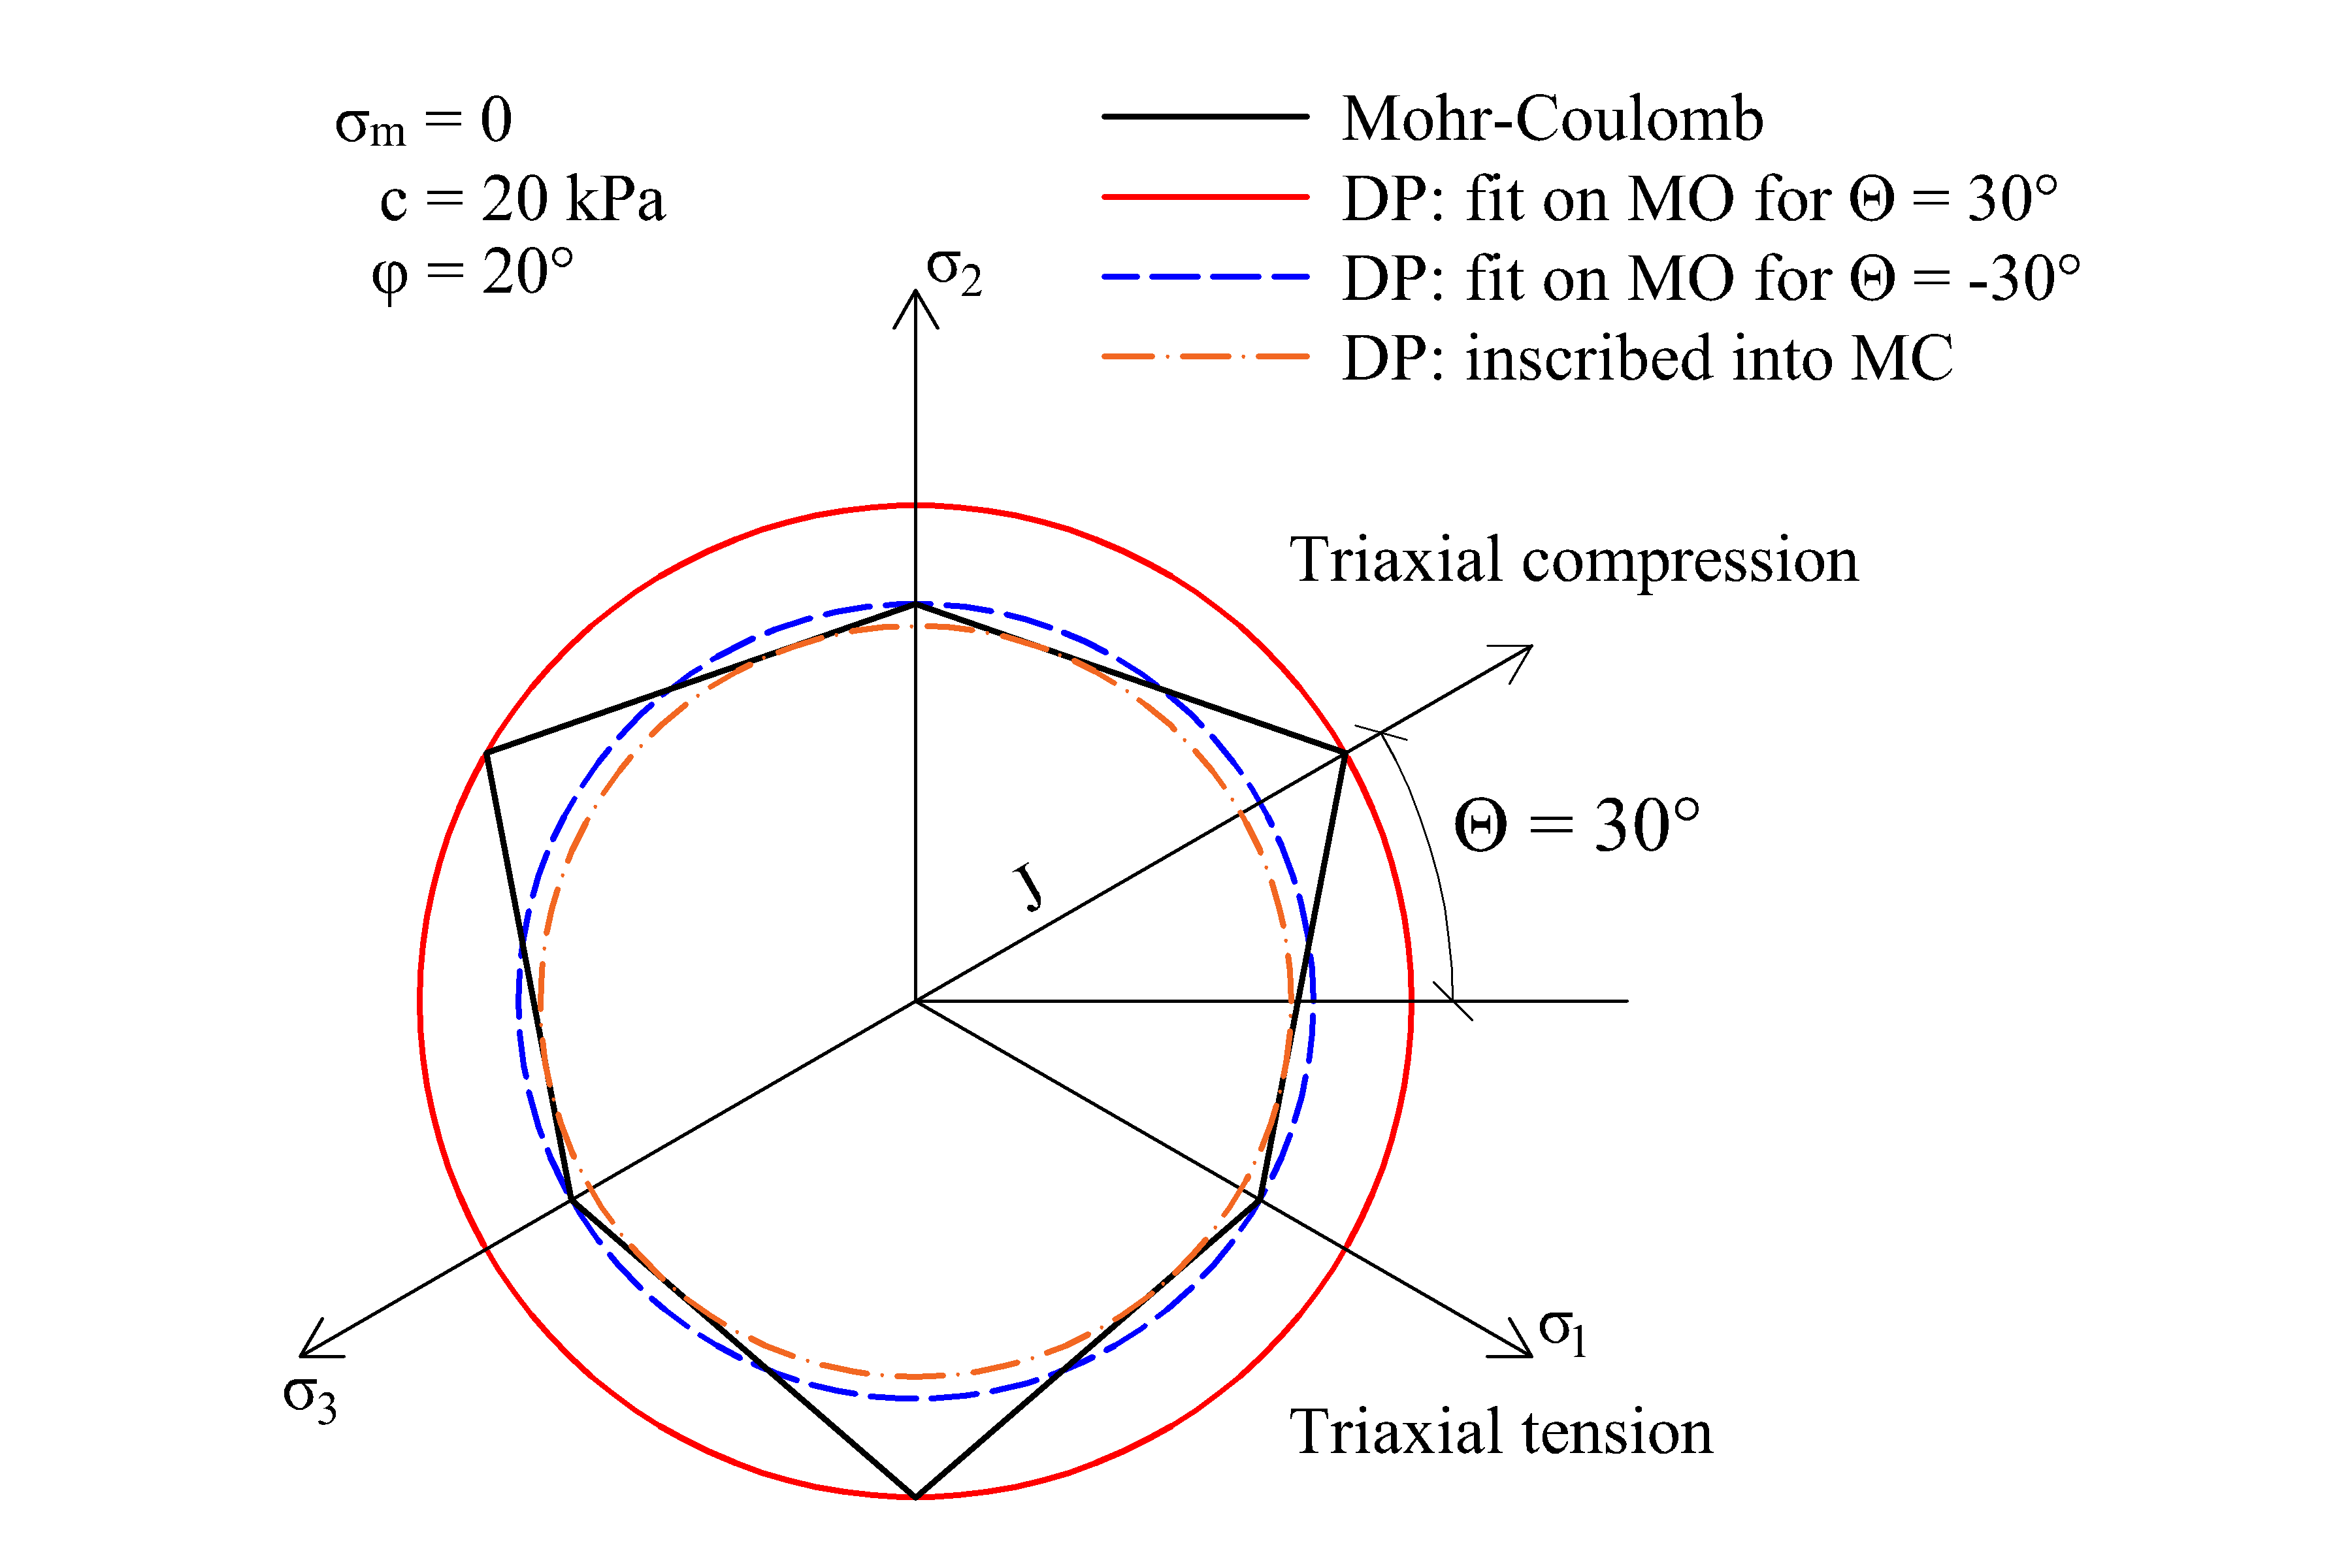
\includegraphics[width=0.8\textwidth, angle=0]{obrazky/drucker-prager_eng.png}
	\caption[Drucker-Prager a Mohr-Coulomb model $T$]{Drucker-Prager and Mohr-Coulomb yield criterion in space of principal stresses. \label{obr:F1}}
\end{figure}

\subsubsection{Drucker-Prager yield surface}\label{sec:drucker-prager_yield_criterion}
\indent

As you can see in section (\ref{sec:drucker-prager_introduction}), Drucker-Prager model extend the von Mises model by including the mean stress in the yield criterion equation, which has the form  

\begin{equation}\label{eq:f_yc}
	F(\sigma) = J + (\sigma_m-c(\kappa_{1}) \cot \varphi(\kappa_{2}) )M_{JP}(\varphi(\kappa_{2})) = 0,
\end{equation}

where $J$ is the second invariant of stress tensor, $\sigma_m$ is the mean stress and $M_{JP}$ is used for approximation to the Mohr-Coulomb model and has more forms dependent on point, which used to be approximated. They are defined as:

\begin{equation}\label{eq:f_J_sigM}
	J = \sqrt{\dfrac{1}{6} \left[(\sigma_{11}-\sigma_{22})^{2} + (\sigma_{11}-\sigma_{33})^{2} + (\sigma_{22}-\sigma_{33})^{2}\right] + \tau_{12}^{2} + \tau_{13}^{2}+ \tau_{23}^{2}},
\end{equation}


\begin{equation}\label{eq:f_sigM}
	\sigma_m = \dfrac{\sigma_{11} + \sigma_{22} + \sigma_{33}}{3}.
\end{equation}

Three different Drucker-Prager cones are in Fig \ref{obr:F1}. First one, red circle, touches Mohr-Coulomb yield criterion at $\theta = 30^\circ$ (triaxial compression) with $M_{JP}$ defined as

\begin{equation}\label{eq:f_Mjp_30}
	M_{JP}^{\theta=30^\circ} = \dfrac{2\sqrt{3}\sin\varphi}{3-\sin \varphi},
\end{equation}

where $\varphi$ is tangle of internal friction. Second, blue circle, match Mohr-Coulomb model at  $\theta = -30^\circ$ (triaxial tension), can be obtained from

\begin{equation}\label{eq:f_Mjp_-30}
	M_{JP}^{\theta=-30^\circ} = \dfrac{2\sqrt{3}\sin\varphi}{3+\sin \varphi},
\end{equation}

and the last, green circle is inscribed, and can be determined by

\begin{equation}\label{eq:f_Mjp_i}
	M_{JP} = \dfrac{\sin(\varphi)}{cos(\theta)-\frac{\sin(\theta)\sin(\varphi)}{\sqrt{3}}},
\end{equation}

\begin{equation}\label{eq:f_theta}
	\theta = \arctan{\frac{\sin{\varphi}}{\sqrt{3}}}
\end{equation}

In the Fig \ref{obr:M1} you can see that, Drucker-Prager model is not defined just by the yield function $F$ but also $G$, which is the plastic potential function. Its purpose is for return to the yield of plasticity, when it is overpassed, and can be written in form 

\begin{equation}\label{eq:G}
	G = J + \left[ \sigma_m - a_{pp} \right] M_{JP}^{PP} = 0,
\end{equation}

where $a_{pp}$ follows from Fig. \ref{obr:M1} when matching $F$ and $G$ for the current value of stress $\sigma$, which gave equation

\begin{equation}\label{eq:app}
	a_{pp} = - \sigma_m^c + ( \sigma_m^c - c\cot\varphi) \dfrac{M_{JP}}{M_{JP}^{PP}}
\end{equation} 

When substituting $a_{pp}$ into the plastic potential function (\ref{eq:G}), it can be rewritten as 

\begin{equation}\label{eq:plastic_potential}
	G = J + \left[ \sigma_m - - \sigma_m + ( \sigma_m^c - c\cot\varphi) \dfrac{M_{JP}}{M_{JP}^{PP}} \right] M_{JP}^{PP} = 0,
\end{equation}

where $M_{JP}^{PP}$ is the gradient of the plastic potential function in $J-\sigma_m$ space (Fig \ref{obr:M1}). When functions of plastic potential and yield function  $M_{JP}^{PP}=M_{JP}$, model becomes associated. $M_{JP}^{PP}$  can be related to the angle of dilatation $\psi$, and can be substituted for $\varphi$ in Equations (\ref{eq:f_Mjp_-30})-(\ref{eq:f_theta}).
 
\subsubsection{Hardening and softening modulus}
\indent

In the model, inspired by the von Mises plasticity model, is implemented derivation of hardening/softening modulus. To that end, we choose multi-linear form of the hardening/softening law for the cohesion $c$ and the angle of internal friction $\varphi$, as shown in Fig. \ref{obr:H}, where also you can see that variation of $c$ and $\varphi$ is a function of deviatoric plastic strain $E_d^{pl}$. Thought the components of vector $\kappa$ may vary for each of the two strength parameters, in the present formulation is assumed a single hardening parameter

\begin{equation}\label{eq:kappa}
	\kappa = \kappa_{1} = \kappa_{2} = E_d^{pl}
\end{equation}

\begin{figure}[h!]
	\centering	
	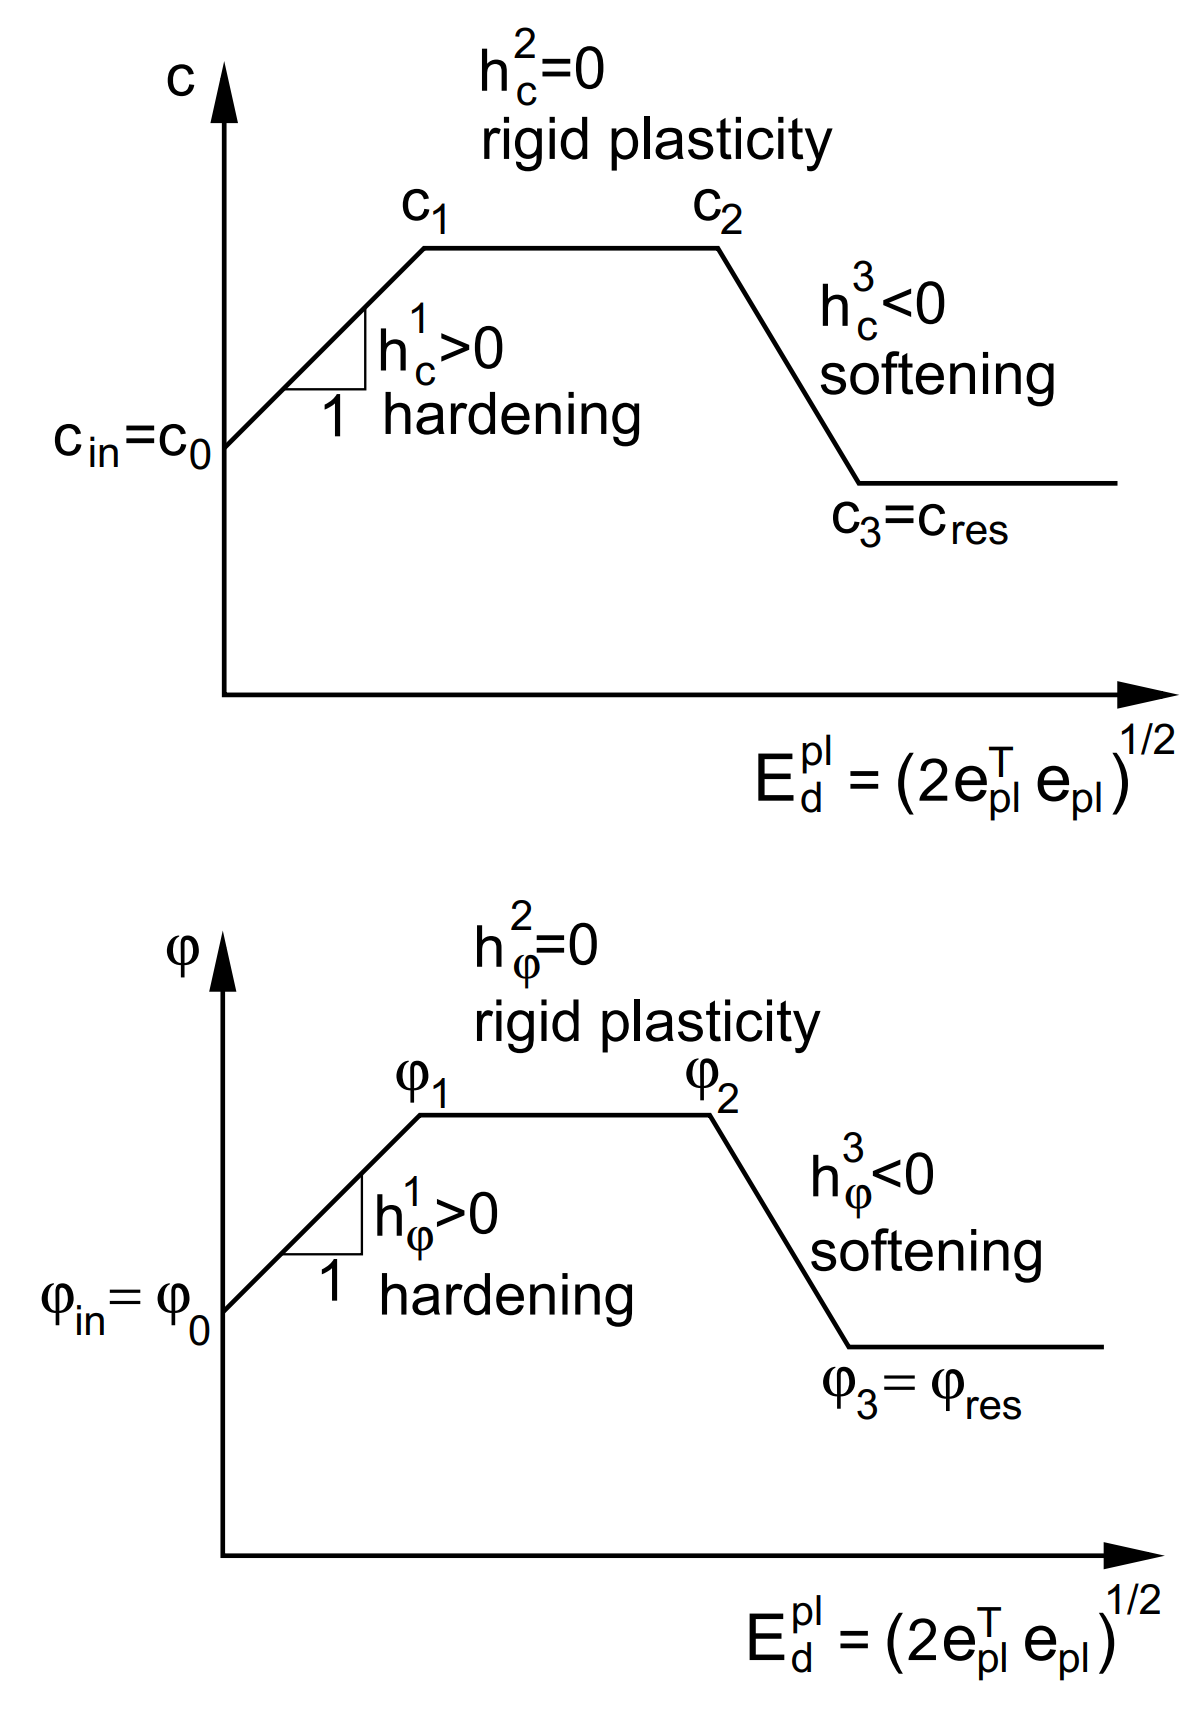
\includegraphics[width=0.8\textwidth, angle=0]{obrazky/hardening_softening_modulus.png}
	\caption[Hardening and softening modulus]{Hardening and softening modulus \cite{geofem}: $c_{in}$ and $c_{res}$, respective $\varphi_{in}$ and $\varphi_{res}$ represent initial and residual values of $c$ and $\varphi$.} \label{obr:H}
\end{figure}
 
Multi-linear formulation suppose that and $n^{th}$ interval in the Fig. \ref{obr:H} is active, then the current strenght parameters can be provided by

\begin{equation}\label{eq:c}
	c = c^{n-1} + h_c^n \left( E_d^{pl} -(E_d^{pl})^{n-1} \right),
\end{equation}

\begin{equation}\label{eq:phi}
\varphi = \varphi^{n-1} + h_\varphi^n\left( E_d^{pl} - (E_d^{pl})^{n-1} \right),
\end{equation}

where $h_c^n$ and $h_\varphi^n$ are the hardening/softening moduli for $c$ and $\varphi$ and can be written in the form


\begin{equation}\label{eq:h_c}
	h_c^n = \dfrac{c^n-c^{n-1}}{(E_d^{pl})^{n}-(E_d^{pl})^{n-1}}
\end{equation}

\begin{equation}\label{eq:h_phi}
 	\varphi_c^n = \dfrac{\varphi^n-\varphi^{n-1}}{(E_d^{pl})^{n}-(E_d^{pl})^{n-1}}
\end{equation}

From \cite{geofem} hardening modulus can be determined by

\begin{equation}\label{eq:H_first}
	H = \left(-\dfrac{\partial F}{\partial \kappa}\right)^T \dfrac{\partial \kappa}{\partial \lambda},
\end{equation}
\newpage
and referring to Fig. \ref{obr:H} and using Eq. (\ref{eq:H_first}) the hardening/softening modulus $H$ assumes the form 

\begin{equation}\label{eq:H}
	H = - \pdv{F}{c} \dv{c}{E_d^{pl}} \dv{E_d^{pl}}{\lambda} - \pdv{F}{\varphi} \dv{\varphi}{E_d^{pl}}, \dv{E_d^{pl}}{\lambda}
\end{equation}

where
\begin{align}
\pdv{F}{\varphi}& = \dfrac{c}{\sin^2\varphi} M_{JP} + (\sigma_m - c\cot \varphi) \dv{M_{JP}}{\varphi},\label{eq:F/phi}\\
\dv{F}{c}& = - \cot \varphi M_{JP},\\
\dv{c}{\kappa}& = \dv{c}{E_d^{pl}} = h_c,\\
\dv{\varphi}{\kappa}& = \dv{\varphi}{E_d^{pl}} = h_\varphi
\end{align}

Derivatives of $M_{JP}$ with respect to $\varphi$ for selected values of $\theta$ are

\begin{align}
	\dv{M_{JP}^{ins}}{\varphi}					& = \dfrac{3\sqrt{3}\cos \varphi}{(3 + \sin^2 \varphi)^{\frac{3}{2}}},\\
	\dv{M_{JP}^{\theta = \ang{-30}}}{\varphi}	& = \dfrac{6\sqrt{3}\cos \varphi}{(1-\sin \varphi)^2},\\
	\dv{M_{JP}^{\theta = \ang{30}}}{\varphi}	& = \dfrac{6\sqrt{3}\cos \varphi}{(1+\sin \varphi)^2}.
\end{align}


When we accept the strain hardening approach, then we can write

\begin{align}
	\dd\varepsilon^{pl}& = \dd\lambda\pdv{G}{\sigma} = \dd\lambda\dfrac{1}{2J}P\sigma,\\
	\dd\kappa& = \dd E_d^{pl} = \sqrt{2(\varepsilon^{pl})^T \text{\textbf{QPQ}} \varepsilon^{pl} } = \dd \lambda = \dv{E_d^{pl}}{\lambda} = 1.\label{eq:dkappa}
\end{align}

With final substitution of Eq. (\ref{eq:F/phi})-(\ref{eq:dkappa}) back into Eq. (\ref{eq:H}), result is searcehd form of the hardening/softening modulus as

\begin{equation}\label{eq:H_final}
	H = h_c \cot\varphi M_{JP} - h_\varphi \left[ \dfrac{c}{\sin^2 \varphi} M_{JP} + (\sigma_m - c \cot \varphi) \dv{M_{JP}}{\varphi} \right].
\end{equation}

\subsubsection{Tangent stiffness matrix}
\indent

The instantaneous tangent stiffness matrix taken from \cite{geofem} is modified stiffness matrix, that take to account with the hardening modulus and the deviatoric plastic strain and has the form

\begin{equation}
	\mathcal{D}^{\textit{cons}} = \mathcal{D} \dfrac{\mathcal{D} n_g n^T \mathcal{D}}{H + n^T \mathcal{D} n_g},
\end{equation}

where $\mathcal{D}$ is the reduced stiffness matrix defined 

\begin{equation}
	\mathcal{D}	= \left[  (\boldsymbol{\text{\textbf{D}}}^{el})^{-1} + \Delta \lambda \pdv{n_g}{\sigma} \right]^{-1},
\end{equation}

where $\textbf{D}^{el}$ is ordinary stiffness matrix. The partial derivatives of the yield function and plastic potential function with respect to stress can be found using the chain rule

\begin{equation}
	n = \pdv{F}{\sigma} = \pdv{F}{\sigma_m} \pdv{\sigma_m}{\sigma} + \pdv{F}{J}\pdv{J}{\sigma},
\end{equation}

\begin{equation}
	n_g = \pdv{G}{\sigma} = \pdv{G}{\sigma_m} \pdv{\sigma_m}{\sigma} + \pdv{G}{J}\pdv{J}{\sigma}.
\end{equation}

In fact, $n$, respective $n_g$, represent normals to the yield respective the plastic potential functions in the stress space. From \ref{eq:f_yc} and \ref{eq:G} can be easily calculated 

\begin{equation}
	\pdv{F}{f\sigma_m} = M_{JP}, \pdv{G}{\sigma_m} = M_{JP}^{PP}, \pdv{F}{J} = \pdv{G}{J} = 1.
\end{equation}

Partial derivatives of stress tensor invariants are model independent with the form 

\begin{equation}
	\pdv{\sigma_m}{\sigma} = \text{\textbf{m}},
\end{equation}

\begin{equation}
	\pdv{J}{\sigma} = \pdv{(\sigma^T\text{\textbf{P}}\sigma)^{\frac{1}{2}}}{\sigma} = \dfrac{1}{2J} \text{\textbf{P}}\sigma.
\end{equation}

With expressions above we can finally get 

\begin{equation}
	\pdv{F}{\sigma} = \dfrac{1}{2J}\text{\textbf{P}}\sigma + \text{\textbf{m}}M_{JP},
\end{equation}

\begin{equation}
	\pdv{G}{\sigma} = \dfrac{1}{2J}\text{\textbf{P}}\sigma + \text{\textbf{m}}M_{JP}^{PP}.	
\end{equation}

As last we need the second derivation of \ref{eq:G} to determine algorithmic tangent stiffness matrix $\mathcal{D}^{cons}$, which has the form 

\begin{equation}
	\pdv{n_g}{\sigma} = \left( \dfrac{3}{2} \right)^{1/2} \dfrac{\sigma^T \text{\textbf{P}} \sigma \text{\textbf{P}}}{(\sigma^T \text{\textbf{P}} \sigma)^{3/2}}.
\end{equation}

\subsubsection{Calculation procedure and implementation}\label{sec:drucker-prager_count}
\indent

Total elastic stress can be calculated as 
\begin{equation}\label{eq:f_sigma}
\sigma = \text{\textbf{D}}^{el} \varepsilon_e,
\end{equation}
where \textbf{D}$^{el}$ is ordinary stiffness matrix and $\varepsilon_e$ is elastic deformation. Calculation is performed in  implicit software \cite{mars}, so model is implemented with increments. Then can be equation modified as

\begin{equation}\label{eq:f_sigma1}
	\sigma^{n+1} = \sigma^n+ \text{\textbf{D}}^{el} \mathrm{d} \varepsilon_e.
\end{equation}

Next step in calculation is find out, if is Eq. (\ref{eq:f_yc}) satisfied, if is, strains ans stresses are stored, and calculation continues with next deformation increment. If yield function exceeded, material behavior become to be from basic elastic to elasto-plastic with hardening. Due to higher amount of the variables, which describe return to the yield of plasticity, is necessary to implement the Jacobian matrix\footnote{Matrix of partial derivations}. There are four material parameters that may vary, when is performed return to yield of plasticity:

\begin{itemize}
	\item $\Delta\lambda$ - Coefficient of plastic flow,
	\item $c$ - Cohesion,
	\item  $\varphi$ - Angle of friction,
	\item $\psi$ - Angle of dilatation.
\end{itemize}

Before of describing Jacobian matrix, we need to find out basic equations, which are used in it and define dependence of all variables. 
Plastic strain increment have the form 

\begin{equation}
	\dd \varepsilon^{pl} = \Delta \lambda \pdv{G}{\sigma},
\end{equation}

and with accepting this flow rule, then increments of yield respective plastic strain int the form 

\begin{align}
	\dd \varepsilon_\nu^{pl} &= \dd \lambda \pdv{G}{\sigma_m} = \Delta \lambda M_{JP}^{PP} \sin \psi,\\
	%\dd e^{pl} &= \dd \lambda \pdv{G}{s} = \dd \lambda \dfrac{\text{\textbf{G}}^{-1}s}{2J}\text{ where } s = \text{\textbf{PQ}}\sigma,\\
	\dd E_{d}^{pl} &= \dd \lambda \pdv{G}{J} = \Delta \lambda,
\end{align}

which further allows writing the corresponding stresses at the end of the $i+1$ load increment as  

\begin{align}
	\sigma_m^{i+1} &= \sigma_m^{tr} - K M_{JP}^{PP} (\sin \psi^{i+1}) \Delta \lambda,\\
	%s^{i+1} &= s^{tr} - 2\mu \Delta \lambda\dfrac{s^{i+1}}{2J^{i+1}} = \dfrac{s^{tr}}{1 + \dfrac{\mu \Delta \lambda}{J^{i+1}}} = s^{tr} \left( 1 - \dfrac{\mu \Delta \lambda}{J^{tr}}   \right),\\
	J^{i+1} &= J^{tr} + \mu \Delta \lambda,
\end{align}

where $K$ is the bulk modulus and $\mu$ represent the elastic shear modulus to avoid misinterpretation with the plastic potential function. Now can be the Jacobian matrix defined.

\begin{itemize}
	\item Primary variables
	
	\begin{equation}
		\lbrace \mathbf{a} \rbrace ^T = \lbrace \Delta \lambda, c^{i+1}, \varphi^{i+1}, \psi^{i+1} \rbrace.
	\end{equation}
	
	\item Residuals
	\begin{equation}
		\lbrace \mathcal{r} \rbrace =  \lbrace \mathcal{F}, \mathcal{C}, \mathrm{\Phi}, \mathrm{\Psi} \rbrace,
	\end{equation}
	where \begin{align}
		\mathcal{F} &= \overbrace{J^{tr}-\mu\Delta\lambda}^{J^{i+1}} + [\overbrace{\sigma_m^{tr}-K M_{JP}^{PP}(\sin \psi^{i+1})\Delta\lambda}^{\sigma_m^{i+1}}-c^{i+1}\cot\varphi^{i+1}]M_{JP}(\sin\varphi^{i+1}),\label{eq:f_yc_lam}\\
		\mathcal{C} &= c^{i+1} - \hat{c} = 0,\label{eq:C_jac}\\
		\mathrm{\Phi} &= \varphi^{i+1} - \hat{\varphi} = 0,\label{eq:phi_jac}\\
		\mathrm{\Psi} &= \psi^{i+1} - \hat{\psi} = 0.
	\end{align}
	Variables $\hat{c}$ and $\hat{\varphi}$ follows Eq.(\ref{eq:c}) and (\ref{eq:phi}) and the current value of dilatation angle $\hat{\psi}$ can be, with help of Rowe's dilatation theory in triaxial compression, written as
	\begin{equation}
		\sin \hat{\psi} = \dfrac{\sin \varphi^{i+1} - \sin \varphi_{cv}}{1_- \sin \varphi^{i+1} \sin \varphi_{cv}},
	\end{equation}
	where $\varphi_{cv}$ is constant-volume friction angle.
	
	\item Local Newton-Raphson method
	\begin{equation}\label{eq:newton_raphson}
		\lbrace a^{i+1} \rbrace _{k+1} = \lbrace a^{i+1}_k \rbrace - [\text{\textbf{H}}]^{-1} \lbrace r \rbrace_k 
	\end{equation}
	
	\item Jacobian matrix $[\textbf{H}]$
	\begin{equation}
		[\text{\textbf{H}}] = \mqty[\pdv{J}{\Delta \lambda} \pdv{\mathcal{F}}{\sigma_m} \pdv{\sigma_m}{\Delta \lambda} & \pdv{\mathcal{F}}{c} & \pdv{\mathcal{F}}{\varphi} + \pdv{\mathcal{F}}{M_{JP}} \pdv{M_{JP}}{\sin \varphi} & \pdv{\mathcal{F}}{M_{JP}^{PP}} \pdv{M_{JP}^{PP}}{\sin \psi}\\
		\pdv{\mathcal{C}}{\hat{c}} = \pdv{\hat{c}}{\Delta \lambda} & \pdv{\mathcal{C}}{c} & 0 & 0\\
		\pdv{\mathrm{\Phi}}{\sin \hat{\varphi}} = \pdv{\hat{\varphi}}{\Delta \lambda} & 0 & \pdv{\mathrm{\Phi}}{\sin \varphi} & 0 \\
		0 & 0 & \pdv{\mathrm{\Psi}}{\sin \hat{\psi}} \pdv{\sin \hat{\psi}}{\sin \varphi} & \pdv{\mathrm{\Psi}}{\sin \psi}]
	\end{equation}
	where partial derivations are
	
	\begin{align}
		&\pdv{J}{\Delta \lambda} \pdv{\mathcal{F}}{\sigma_m} \pdv{\sigma_m}{\Delta \lambda}  = -\mu - K M_{JP}^{PP}M_{JP},\\
		&\pdv{\mathcal{F}}{c} = -M_{JP}\tan\varphi,\\
		&\pdv{\mathcal{F}}{\varphi} + \pdv{\mathcal{F}}{M_{JP}} \pdv{M_{JP}}{\sin \varphi} = M_{JP} \dfrac{c}{\sin^2\varphi \cos\varphi} + \left( \sigma_m \dfrac{c}{\tan \varphi} \right) \dv{M_{JP}}{\sin \varphi}, \\
		&\pdv{\mathcal{F}}{M_{JP}^{PP}} \pdv{M_{JP}^{PP}}{\sin \psi} = -K \Delta \lambda \dv{M_{JP}^{PP}}{\sin \psi},\\
		&\pdv{\mathcal{C}}{\hat{c}} = \pdv{\hat{c}}{\Delta \lambda} = -h_c, \\
		&\pdv{\mathcal{C}}{c} = 1,\\
		&\pdv{\mathrm{\Phi}}{\sin \hat{\varphi}} = \pdv{\hat{\varphi}}{\Delta \lambda} = -\cos(\varphi) h_{\varphi},\\
		&\pdv{\mathrm{\Phi}}{\sin \varphi} = 1,\\
		&\pdv{\mathrm{\Psi}}{\sin \hat{\psi}} \pdv{\sin \hat{\psi}}{\sin \varphi} = -\dfrac{1 - \sin^2\varphi_{cv} }{1-\sin \varphi \sin \varphi_{cv}},\\
		&\pdv{\mathrm{\Psi}}{\sin \psi} = 1.
	\end{align}
	
	Derivation of $M_{JP}$ with respect to $\sin \varphi$ is not writed in exact form due to variable equation of $M_{JP}$ (\ref{eq:f_Mjp_-30})-(\ref{eq:f_Mjp_i}).
	
	\item Initial conditions
	
	\begin{align}
		\lbrace a_0 \rbrace^T &= \lbrace 0, c^i, \sin \varphi^i, \sin \psi^i \rbrace,\\
		\lbrace r_0 \rbrace^T &= \lbrace J^{tr} + (\sigma_m^{tr}-c^i\cot\varphi^i)M_{JP}(\sin\varphi^i), 0, 0, 0 \rbrace.
	\end{align}
	
\end{itemize} 

\subsubsection{Apex problem}
\indent

The implementation above is applicable for calculation the trial stress when returning back to the yield of plasticity in the direction of plastic strain vector. In the Fig \ref{obr:apex_cones} you can see cones $K_\varepsilon$, which follows direction of the plastic strain vector, and $K_\sigma$, which show the admissible stress domain. Its obvious that, if is standard stress point in region $K_\sigma$, material behaviors is elastic, when it is outside of $K_\sigma$ but also outside of $K_\varepsilon$, computation is performing regular stress return. But the non-associated flow rule restrict the plastic strain increment to belong in the cone $K_\varepsilon$ (Eq. \ref{eq:eps_apex}), so if it belong to it, stress should be returned to apex point. That situation may occur in two cases (Fig. \ref{obr:apex_return}): $(a)$ right after load increment, bud also $(b)$ when performing regular stress return, due change of material parameters. Such a situation can be referred as an "apex problem". 

\begin{equation}\label{eq:eps_apex}
	\dot{\varepsilon}_v \geq M_{JP}^{PP} \dot{E}_d^{pl}.
\end{equation}

In the literature we can find two different stands for performing apex return with:

\begin{itemize}
	\item constant material parameters,
	\item hardening/softening material.
\end{itemize}
At the first case, stress point just return to the apex (Fig.\ref{obr:apex_cones}), so stress form is

\begin{equation}\label{eq:sigPL}
	\sigma^{i+1} = 3c^{i+1} \cot \varphi^{i+1} \textbf{m}.
\end{equation}

In \cite{geofem} author show a variational form of the flow rule to show through the concept of bi-potentials that the vector of plastic strain increments for the apex problem is provided by

\begin{equation}\label{eq:epsPL}
	\Delta\varepsilon^{pl} = (\textbf{D})^{-1}( \sigma^{tr} - 3 c^{i+1} \cot \varphi^{i+1} \textbf{m} )
\end{equation}

under condition



\begin{equation}\label{eq:flow_condition}
\dfrac{1}{G} M_{JP}^{PP} J^{tr} - \dfrac{1}{K} (\sigma_m^{tr} - c^i \cot \varphi^i) < 0.
\end{equation}

Note that Eq. (\ref{eq:epsPL}) is essentially linearized from of a Eq. (\ref{eq:sigPL}).

\begin{figure}[h!]
	\centering	
	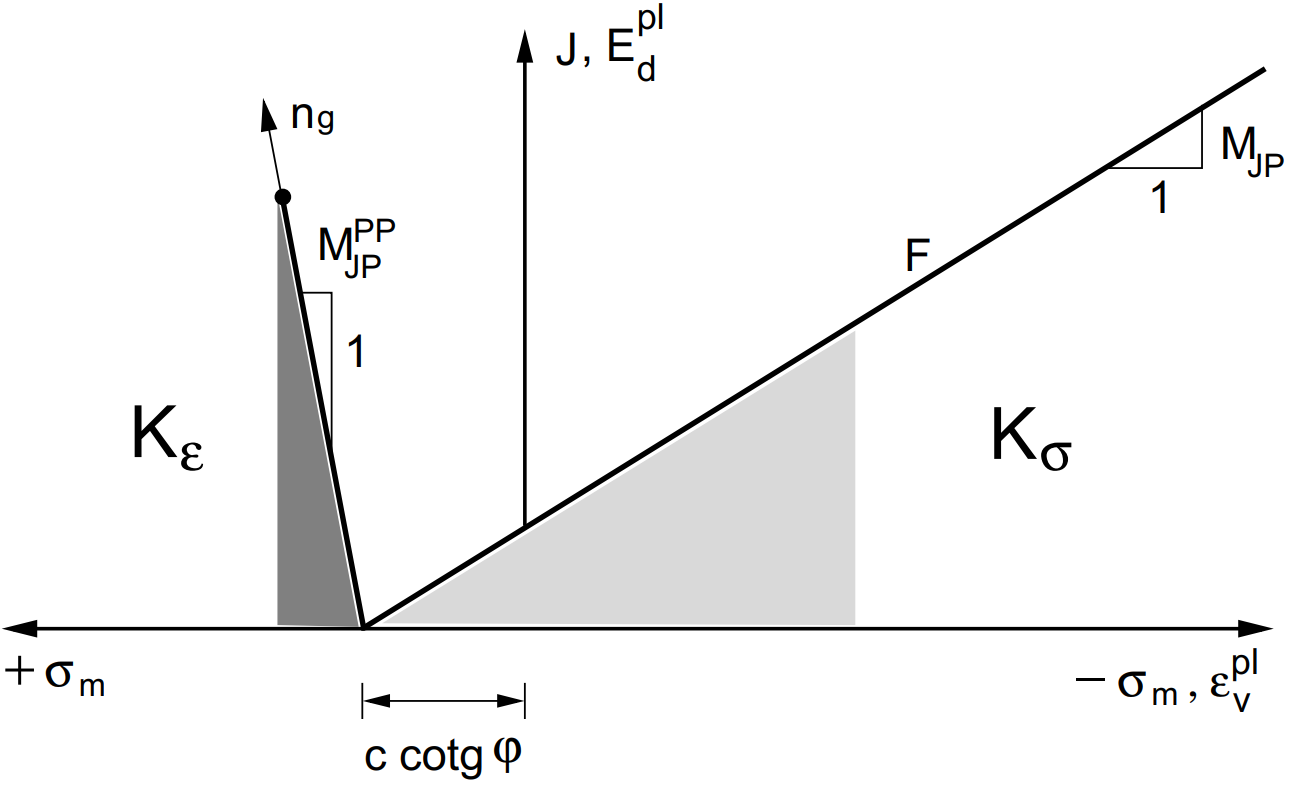
\includegraphics[width=0.8\textwidth, angle=0]{obrazky/apex_cones.png}
	\caption[Apex abmissible regions]{Apex admissible regions for stresses and plastic strain rates \cite{geofem}.} \label{obr:apex_cones}
\end{figure}


\begin{figure}[h!]
	\centering	
	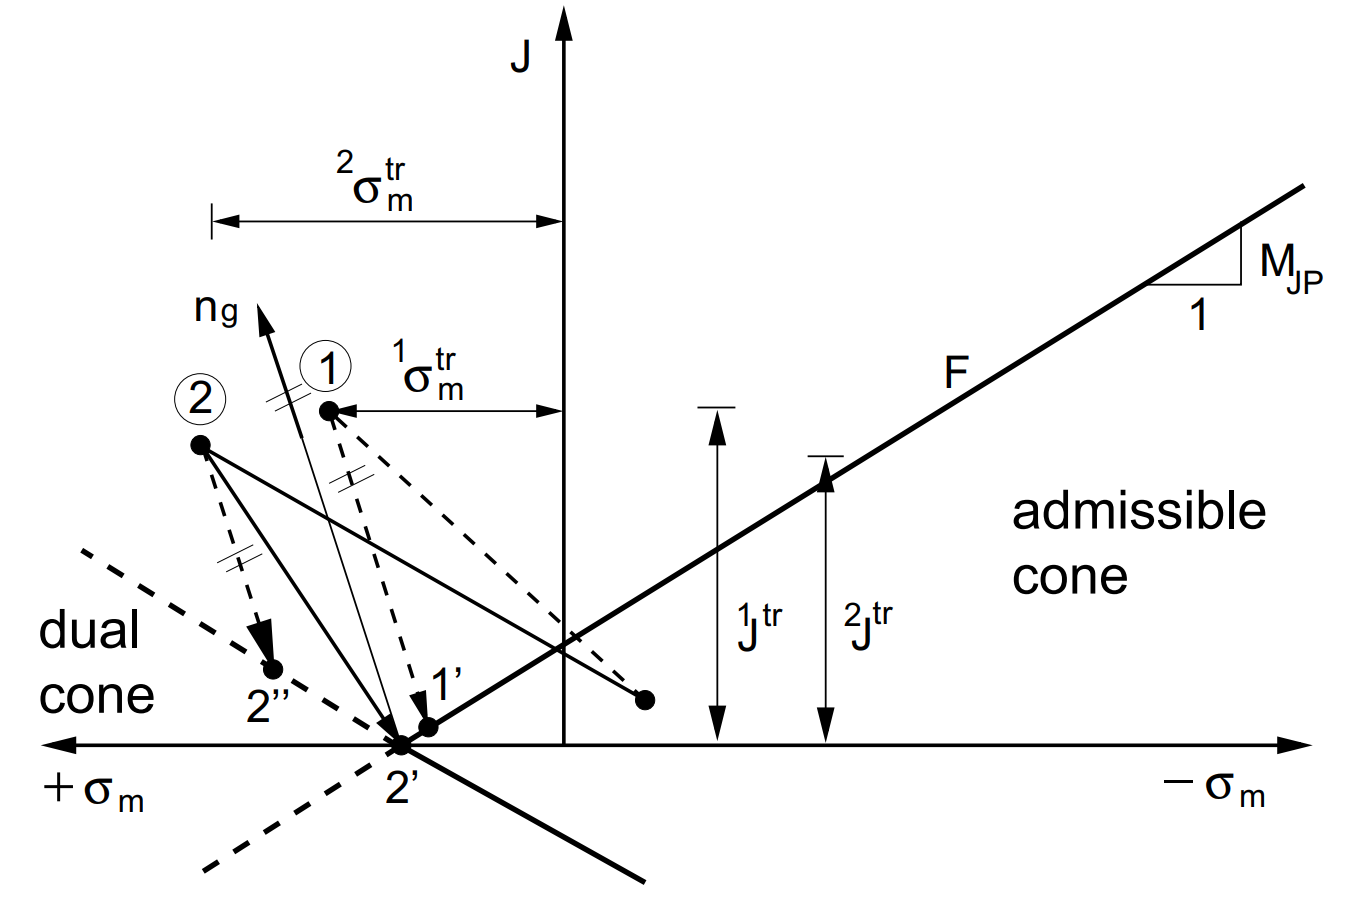
\includegraphics[width=0.8\textwidth, angle=0]{obrazky/apex_recursive_return.png}
	\caption[Apex return]{Apex regular and singular return \cite{geofem}: .} \label{obr:apex_return}
\end{figure}


If we choose second approach of assuming hardening/softening material, we need to update $c$ and $\varphi$ with apex return. Procedure is similar to the regular plasticity return, but with different equations. Before proceeding, we recall that the strain hardening hypotheses is adopted with a single hardening/softening parameter $\kappa$ with form

\begin{equation}\label{eq:hardening_parameter}
	\dot{\kappa} = \dot{E}_d^{pl}
\end{equation}

With Eq. \ref{eq:hardening_parameter} we can reach incremental nonlinear equation with form

\begin{equation}
	\mathcal{E} = \Delta E_d^{pl} - \overbrace{\sqrt{2(\Delta \varepsilon^{pl})^T \textbf{QPQ}\Delta\varepsilon^{pl}} }^{\Delta \hat{E}_d^{pl}}=0
\end{equation}

which would be solved simultaneously with Eq.(\ref{eq:C_jac}) and (\ref{eq:phi_jac}). Note that the increment of plastic strain given by Eq. (\ref{eq:epsPL}) is a function of current strength parameters

\begin{equation}
	\Delta\varepsilon^{pl} = \Delta\varepsilon^{pl} (c^{i+1}, \varphi^{i+1}).
\end{equation}

Due to analogy with the regular return to the yield surface we can also use Newton-Raphson method (Eq.(\ref{eq:newton_raphson})). The calculation procedure is defined:

\begin{itemize}
	\item Primary variables
	
	\begin{equation}
		\lbrace a \rbrace^T = \lbrace \Delta E_d^{pl}, c^{i+1}, \varphi^{i+1} \rbrace.
	\end{equation}
	
	\item Residuals
	
	\begin{equation}
		\lbrace r \rbrace ^T = \lbrace \mathcal{E}, \mathcal{C}, \mathrm{\Phi} \rbrace
	\end{equation}
	
	\item Jacobian Matrix [\textbf{H}]
	
	\begin{equation}
		[\text{\textbf{H}}] = \mqty[\pdv{\mathcal{E}}{\Delta E_d^{pl}} & \pdv{\mathcal{E}}{\Delta\varepsilon^{pl}}^T \pdv{\Delta\varepsilon^{pl}}{c} & \pdv{\mathcal{E}}{\Delta\varepsilon^{pl}}^T \pdv{\Delta\varepsilon^{pl}}{\sin \varphi}\\
		\pdv{\mathcal{C}}{\Delta E_d^{pl}} = \pdv{\mathcal{C}}{\Delta \lambda} & \pdv{\mathcal{C}}{c} & 0 \\
		\pdv{\mathrm{\Phi}}{\Delta E_d^{pl}} = \pdv{\mathrm{\Phi}}{\Delta \lambda} & 0 & \pdv{\mathrm{\Phi}}{\sin \varphi}]
	\end{equation}
	\newpage
	with partial derivations 
	
	\begin{align}
		&\pdv{\mathcal{E}}{\Delta E_d^{pl}} = 1,\\
		&\pdv{\mathcal{E}}{\Delta\varepsilon^{pl}}^T \pdv{\Delta\varepsilon^{pl}}{c} =  -\dfrac{2}{E_d^{pl}} e_{pl}^T (-3\cos\varphi^{i+1}\textbf{m}) = \dfrac{6\cos\varphi^{i+1}}{E_d^{pl}} e_{pl}^T \textbf{m},\\
		&\pdv{\mathcal{E}}{\Delta\varepsilon^{pl}}^T \pdv{\Delta\varepsilon^{pl}}{\sin \varphi} = \pdv{\Delta\varepsilon^{pl}}{c} =  -\dfrac{2}{E_d^{pl}} e_{pl}^T (-3c^{i+1}\textbf{m}) = \dfrac{6\cos c^{i+1}}{E_d^{pl}} e_{pl}^T \textbf{m} ,\\
		&\pdv{\mathcal{C}}{\Delta E_d^{pl}} = \pdv{\mathcal{C}}{\Delta \lambda} =  -h_c,\\
		&\pdv{\mathcal{C}}{c} = 1,\\
		&\pdv{\mathrm{\Phi}}{\Delta E_d^{pl}} = \pdv{\mathrm{\Phi}}{\Delta \lambda} = -\cos(\varphi) h_{\varphi} ,\\
		&\pdv{\mathrm{\Phi}}{\sin \varphi} = 1.
	\end{align}
	
	where $e_{pl}$ is deviatoric part of strain tensor. 
		
	\item Initial conditions
	\begin{equation}
		\lbrace a_0 \rbrace^T = \lbrace 0, c^i, \varphi^i\rbrace,
	\end{equation}
	
	\begin{equation}
		\lbrace r_0 \rbrace^T = \lbrace \sqrt{2(\Delta \varepsilon^{pl})^T(c^i, \varphi^i) \textbf{QPQ}\Delta\varepsilon^{pl}(c^i, \varphi^i)}, 0, 0\rbrace.
	\end{equation}
\end{itemize}
 


\cleardoublepage
%\mbox{}
\thispagestyle{empty}
%\newpage
\section{Results}


\cleardoublepage
\thispagestyle{plain}
\section*{Conclusion}
\addcontentsline{toc}{section}{\protect\numberline{}Conclusion}
\indent

%\thispagestyle{empty/plain/headings/myheadings}


\cleardoublepage
%\input{./kapitoly/kapitola7}

}
\setstretch{1.2}{
	\clearpage
	%\input{priloha0}
	\clearpage
	%\input{priloha1}
}


\cleardoublepage

\bibliography{thesisbiblio}


\begin{comment}
	Obsah...

\begin{thebibliography}{99}
	\bibitem{anchors-ACI-318M}
	ACI (2008). ACI 318M-08 Building code requirements for structural concrete. ACI
	
	\bibitem{hilti_anchors}
	Post-installed anchors. Hilti - mechanical vs adhesive anchors [online]. [cit. 2018-04-21].  
	
	Available from: $https$:$//ask.hilti.com/article/mechanical$-$vs$-$adhesive$-$anchors/rysrkl$
	
	\bibitem{adhesive_anchors}
	Sherief S.S. Sakla, Ashraf F. Ashour, \textit{Prediction of tensile capacity of single adhesive anchors using neural networks},	Computers $\&$ Structures \textbf{83} (2005) 1792-1803.
	
	\bibitem{thermosetting_polymers}
	PASCAULT, Jean-Pierre. Thermosetting polymers. New York: Marcel Dekker, c2002. Plastics engineering (Marcel Dekker, Inc.), 64. ISBN 08-247-0670-6.
	
	\bibitem{mars}
	More info on official site: 
	$http://mars.es3inc.com/www_es3inc_com/marssolver/$
	
	\bibitem{geofem}
	Prof. Ing. Michal Šejnoha, Ph.D., DSc. GEO FEM - Theoretical manual: A computer program for nonlinear finite element analysis of geotechnical problems. 2009, FINE Ltd. 1999-2009.
    	
\end{thebibliography}
\end{comment}
\end{document}
